% http://www.idsc.ethz.ch/education/theses-semester-projects.html
% IDSC LaTeX Thesis Template
% 
% Author(s):	Eric Müller
% 				Institute for Dynamic Systems and Control
% 				Swiss Federal Institute of Technology (ETH) Zurich
% 
% Created:		2004/04/02  (Eric Mueller)
% 
% Notes: Has been tested on Windows 7 + MikTeX + TeXnicCenter
%
% Revisions: 	2009/05/29  (Soren Ebbesen)
% 				    2011/03/22	(Soren Ebbesen)
%             2013/03/08	(Soren Ebbesen)
%             2014/03/13	(Soren Ebbesen)
% ______________________________________________________________________________
\documentclass[10pt,twoside,a4paper,fleqn]{report}


\usepackage[english,st]{ethidsc} % Special IDSC styles and commands      	
								 % {german}/english: language of headings, etc.
								 % {st}/bt/mt: {semester}/bachelor/master thesis
							
% Page header (don't change)____________________________________________________
\setlength{\parindent}{0em}                 % Disable parindent
\rhead[\nouppercase{\rightmark}]{\thepage}  % Special headings
\lhead[\thepage]{\nouppercase{\leftmark}}   % Special headings
\cfoot{}                                    % Special headings


% Title page (please fill in)___________________________________________________
\title{Tropical Cyclone Tracking with varying parameter thresholds}


\studentA{Jan Engelmann}
\ethidA{15-936-784}
\semesterA{3}
\emailA{enjan@ethz.ch}

%\studentB{Second Student}
%\ethidB{12-345-678}
%\semesterB{9}
%\emailB{second@student.ethz.ch}

\supervision{Bernhard Enz\\ Prof. Dr. Ulrike Lohmann}
\date{November 2020}


\infopage
\declaration

% Begin document________________________________________________________________
\begin{document}

\maketitle 							% Create title page


% Preamble______________________________________________________________________

\pagenumbering{roman} 				% Begin roman page numbering (i,ii,...)

% Table of contents

 \setcounter{tocdepth}{2}
 \tableofcontents

%---------------------------------------------------------------------------
% Abstract


\chapter*{Abstract}
 \addcontentsline{toc}{chapter}{Abstract}
Tropical Cyclone (TC) tracking in simulation data requires parameter thresholds that specify the expected intensity of these characterising variables. This results in assumptions for a specific climate model that may or may not lead to a successful tracking of TCs. With the purpose of being able to run the algorithm with different parameter assumptions, an existing algorithm was optimised and a 60-fold speedup reached. This enabled experimentation with numerous different threshold combinations. It was found that correctly adjusting the warm core criterion is of central importance since it balances the unwanted tracking of noise with the desired early discovery of tropical cyclones. Furthermore, including a requirement in regards to the minimum sea surface temperature during TC genesis made the algorithm more robust. The analysis of the vorticity criterion suggested further investigation of its effectiveness. Finally, matching tracks across threshold combinations significantly improved the understanding of parameter interplay and the tracking of TCs across their lifetime.

% Chapters______________________________________________________________________



\pagestyle{fancy}               	% Fancy headings
\pagenumbering{arabic}				% Begin arabic page numbering (1,2,...)

\chapter{Introduction}\label{sec:introduction}
\begin{enumerate}
\item DONE Tcs are relevant for society due to their changing intensity and more people living on the coast
\item They exhibit interesting physics (tiefdrucksysteme mit Warmcore)
\item They are studied analytically, with field experiments and with simulations
\item Here their climatology is analyzed by analyzing simulation data
\end{enumerate}
Tropical cyclones also known as Hurricanes or Typhoons are storms of extreme nature in many regards. Not only are they the most deadly and expensive natural catastrophes in the United States but also their physics is quite challenging with many open questions remaining.\cite{emanuel-summ}
Finally they are very likely to play a crucial role in the global heat balance and moisture circulation.\cite{moisture-transport}\cite{global-heat}

\section{Impact on society}\label{sec:society}
While tropical cyclones form and intensify above the ocean, they have the largest impact on society during landfall. The damage happens due to a combination of strong winds and catastrophic storm surges. On average hurricanes inflict normalized damages of about \$10-billion/year in the United States.\cite{damage-norm} A single strong storm can cause thousands of deaths. Hurricane Katrina e.g. in 2005 took the lives of over 1200 people.\cite{hurr-2005}
Due to these enormous implications for society and opportunities to save lives and money, active research is happening on tropical cyclone impact reduction. With an unsure impact of climate change on tropical cyclone frequency and intensity and a trend of urbanization on the American east-coast, improving the understanding of tropical cyclones is of great importance.

\section{Underlying Physics}\label{sec:physics}
Tropical Cyclones can be classified using the Saffir-Simpson wind scale. It is defined by the maximum wind observed in the cyclone.This is motivated by the strong correlation between wind speeds and the inflicted damages.\cite{simpson} 
\begingroup
\setlength{\tabcolsep}{10pt} % Default value: 6pt
\renewcommand{\arraystretch}{1.5} % Default value: 1
\begin{table}[hbt!]
\centering
\begin{tabular}{|c|c|c|c|c|}
\cline{1-2} \cline{4-5}
\multicolumn{2}{|c|}{\textbf{Tropical Cyclones}} &  & \multicolumn{2}{c|}{\textbf{Other tropical low pressure systems}} \\ \cline{1-2} \cline{4-5} 
category     & wind speed {[}m/s{]}     &  & name                & wind speed {[}m/s{]}               \\ \cline{1-2} \cline{4-5} 
1 & 33--42    &  & tropical depression & $\leq$ 17 \\
2 & 43--49    &  & tropical storm      & 18--32    \\
3 & 50--58    &  &                     &           \\
4 & 58--70    &  &                     &           \\
5 & $\geq$ 70 &  &                     &           \\ \cline{1-2} \cline{4-5} 
\end{tabular}
\caption{Simpson scale defined by 1-minute maximum sustained winds}
\label{tab:simpson-scale}
\end{table}
\endgroup

\begin{enumerate}
\item DONE Classification between tc, tornado, tropical depression...
\item Mention climatology and categorisation
\item Genesis criteria
\item Carnot Cycle
\item Shortly mentioning WISHE Paradigm
\item Mention 1 or 2 of Heini Wernlis Publications
\item use emanuel review paper and cloud dynamics course material
\end{enumerate}


\section{Previous work on TC Tracking}\label{sec:tracking}
\begin{enumerate}
\item Mention work of Christoph Raible/Raibler from Bern regarding TC Tracking
\item See what Heini Wernli has done
\end{enumerate}
\cleardoublepage
\chapter{Data and Methods}
\label{sec:methods}
The purpose of this project was to evaluate the parameter thresholds for
tracking TCs in ICON simulation data. In the following section the settings
used for generating the simulation data and the algorithm itself will be
explained.
\section{Simulation Data}
\label{sec:data}
\subsection*{ICON Model}
The Icosahedral Nonhydrostatic Model (ICON) is developed by the German Weather
Service (DWD), the Max Planck Institute for Meteorology and several partner
institutes. As the name implies the grid is in a first step generated by
mapping the earths surface to an Icosahedron (platonic solid with 20
equilateral triangles as faces). The faces are then split up into smaller
triangles in order to achieve the desired resolution. The model then delivers
all typical meteorological quantities on this grid.
The model uses the fully compressible and non-hydrostatic version of the Euler
equations for the fundamental transport processes. Physical processes which
cannot be resolved with the grid size are then parametrised by using complex
functions that take into account the grid box mean values of the model
variables. Physical processes which need to be treated in this way include
solar and thermal radiation, cloud microphysics and turbulent transfer above
the earth's surface.\cite{dwd-icon}

\subsection*{Analysed simulation output}
The North Atlantic basin with its surrounding area ( TODO xx1 - xx2 lon and yy1
- yy2 lat) % TODO find out exact domain 
was simulated from the beginning of May until the beginning of December. The
output data is saved for every six hours.
Two different kinds of time lagged ensembles were used. Both used ERA5
reanalysis data for the initial weather state and the monthly boundary
conditions. The first however, labeled "ref", used the first day of each month
at 6:00 a.m. (TODO !confirm with Bernhard ) % TODO confirm time lagged ensemble with bernhard
as the monthly boundary conditions. The second ensemble, labeld "rm", used
monthly rolling mean boundary conditions based on the same reanalysis data.
The members within each of these two ensembles were created by varying the
initial weather state of the simulation. Namely each of the first 10 days of
May were used as initial conditions for a separate simulation run.
The output data from each run is mapped from the icosahedral to a
Latitude-Longitude grid in order to facilitate distance calculations.
Finally this results in 20 separate simulation runs that can be searched for
TCs.
%TODO RENAME STEPS TO TRACKING AND STITCHING AND THEN EXPLAIN
%TODO mention the amazing job I did in regards to vectorization
\section{Algorithm}
An existing algorithm developed by Bernhard Enz and inspired by \cite{orig-tracking} was improved in regards to runtime, robustness and
readability. The gained speed was used in order to run the algorithm on the
same simulation data but with different threshold values that decide wether a
TC was found or not. By comparing the different results reasonable thresholds
and the importance of the different criteria were determined.\newline
The algorithm consists of two steps. In the first step the TC candidates are
found for each time step without taking into account if a storm already existed
in the previous time-step. Afterwards all entries are analysed and connected to
TC tracks if they lie close to each other temporally and spatially. Both steps
will be explained in the following sections.
\subsection{TC candidate search}
TC candidates are found by searching the simulated domain using several
criteria. They are summarised in Tab.~\ref{tab:search-algo-summ} and will be
explained in detail in the following sections.
\begin{table}[h]
	\centering
	\begin{tabular}{|l|l|}
		\hline
		\textbf{criterion}          & \textbf{parameters} \\ \hline
		sea level pressure minimum  & slpdis              \\
		minimal vorticity threshold & vormin              \\
		warm core criterion         & temdif, temdis      \\ \hline
	\end{tabular}
	\caption{Each criterion can be adjusted by changing its characterising
		parameter}
	\label{tab:search-algo-summ}
\end{table}

\subsubsection*{Sea Level Pressure Minimum}
As outlined in Sec.~\ref{sec:physics} TCs are low pressure systems. In fact
some of the lowest pressures on earth were measured inside the eyes of TCs.
Therefore the first step to finding TC candidates for a specific time-step is
locating the sea level pressure minima. Here enormous speed up was achieved by
replacing the previous manual minimum finding algorithm with a vectorised
version from the image processing library scikit-image~\cite{scikit-image}.
This function finds the local minima and requires them to be a certain distance
apart. The stronger minimum is kept if two candidates are within the specified
distance \textbf{slpdis}. The resulting minima are then further
analysed.
\subsubsection*{Minimal Vorticity Threshold}
If the vorticity at a pressure minimum is below the minimum threshold
\textbf{vormin} it is discarded as a potential TC candidate.

\subsubsection*{Warm Core Criterion}
The last qualifying characteristic is the warm core structure. The temperature
at the height of 300~hPa in the pressure minimum is co1mpared to the average
temperature of the surrounding area at the same height. The form and strength
of this warm core requirement can be adjusted by using the parameters
\textbf{temdif} and \textbf{temdis}. The former corresponds to the required
temperature difference between the center of the storm and its environment.
Only storms that have a warm core that is at least \textbf{temdif} degrees
warmer than the environment, are kept as valid TC candidates. The latter
specifies the side-length of the square with the storm in the middle which is
defined as environment.
\subsubsection*{Saving of TC information}
At the end of each time-step the remaining candidates are saved with their
corresponding date, time, position, maximum windspeed and sea level pressure in
the center.

\subsection{Creating TC tracks from previously found TC candidates}
The TC tracks are created by checking the candidates for each time-step and
comparing them to currently active TCs. At the beginning of each new time-step
previously active TCs that were interrupted are archived if they lived for at
least 18 hours and deleted otherwise. Then for each entry it is checked which
previous TC is within its maximum travel distance. This distance is set to
72~kilometres since a TC with a top speed of 20 m/s can travel this far within
6 hours. If several entries could have been reached by the same active TC, the
entry with the lower sea level pressure is added to the track and the other
entries are discarded. If no active TC within range of the entry is found a new
active TC is created. Each TC is finally assigned a unique integer for
identification.

\subsection{Varying parameter thresholds}
Naturally the results of the algorithm depend on the choice of the five
parameters from Tab.~\ref{tab:search-algo-summ}. In order to answer the
research question of this project the algorithm was run for different
combinations of these parameters. For instance all combinations of the values
in Tab.~\ref{tab:param_combos} were used.

\begin{table}[ht]
	\centering
	\begin{tabular}{|l|l|l|}
		\hline
		\textbf{parameter} & \textbf{unit} & \textbf{values}        \\ \hline
		slpdis             & m             & 25000, 50000, 100000   \\
		vormin             & 1/s           & 1e-6, 1e-5, 1e-4       \\
		temdif             & K             & 0.5, 0.75,1,1.25       \\
		temdis             & m             & 100000, 200000, 400000 \\ \hline
	\end{tabular}
	\caption{An exemplary list of parameters which results in 108 (=3*3*4*3) combinations }
	\label{tab:param_combos}
\end{table}
In summary, the algorithm is run with every parameter set on all of the 20
simulation runs.

\section{Tracking Data Analysis}
\subsection{Algorithm output data format}
The output of the algorithm is a pandas dataframe with one row per unique TC per timestep. Its columns are described in Tab.~\ref{tab:output-data}.
\begingroup
\begin{table}[]
	\centering
	\begin{tabular}{| p{0.3\linewidth} | p{0.27\linewidth} | p{0.38\linewidth }|}
		\hline
		                              &                              &                                                                                        \\[-0.5em]
		\textbf{information}          & \textbf{columns}             & \textbf{description}                                                                   \\[5pt] \hline
		                              &                              &                                                                                        \\[-0.5em]
		timestamp                     & date                         & time and date of the TC entry                                                          \\[5pt]
		position                      & lon\_idx, lat\_idx, lon, lat & position of the found TC in longitude/latitude grid indices and coordinates            \\[5pt]
		intensity                     &
		maxwind, curr\_cat, cat       &
		maximum wind within a 100km distance, snapshot category at the current time, maximum category of the corresponding TC                                 \\[5pt]
		parameter combination         & param\_id                    & id of the parameter combination used for tracking                                      \\[5pt]
		unique TC identifier          & tc\_id                       & unique TC identifier across all parameter combinations and simulation runs             \\[5pt]
		simulation run                & mem, exp                     & variables specifying the member and boundary conditions of the analysed simulation run \\[5pt]
		genesis sea level temperature &
		genesis\_sst                  &
		genesis sea level temperature of the particular TC, identical across all time entries of a TC.                                                        \\[5pt] \hline
	\end{tabular}
	\caption{description of the columns of the output pandas dataframe \cite{pandas}}
	\label{tab:output-data}
\end{table}
\endgroup

\subsection{Filtering out noise}
After the tracking and stitching steps are completed, the algorithm results can
still be improved by filtering the results. The largest improvement was
achieved by requiring a certain sea surface temperature at TC genesis.
\subsubsection*{Sea Surface Temperature Criterion}
As outlined in Sec.~\ref{sec:physics} the TCs need warm ocean water as an
energy source, especially when they form. It has been shown that the large
majority has a SST over 25.5\degree C \cite{sst-paper}. Therefore it is
expected that no reasonable TCs are filtered out when requiring a genesis SST
of at least 24\degree C. However as can be seen in Fig.~\ref{fig:sst-effect}
a large part of the unwanted tracks in the North of the domain are removed.
% TODO use figures here and in general with reasonable and elaborated parameters only
\begin{figure}[ht]
	\begin{minipage}[t]{0.48\textwidth}
		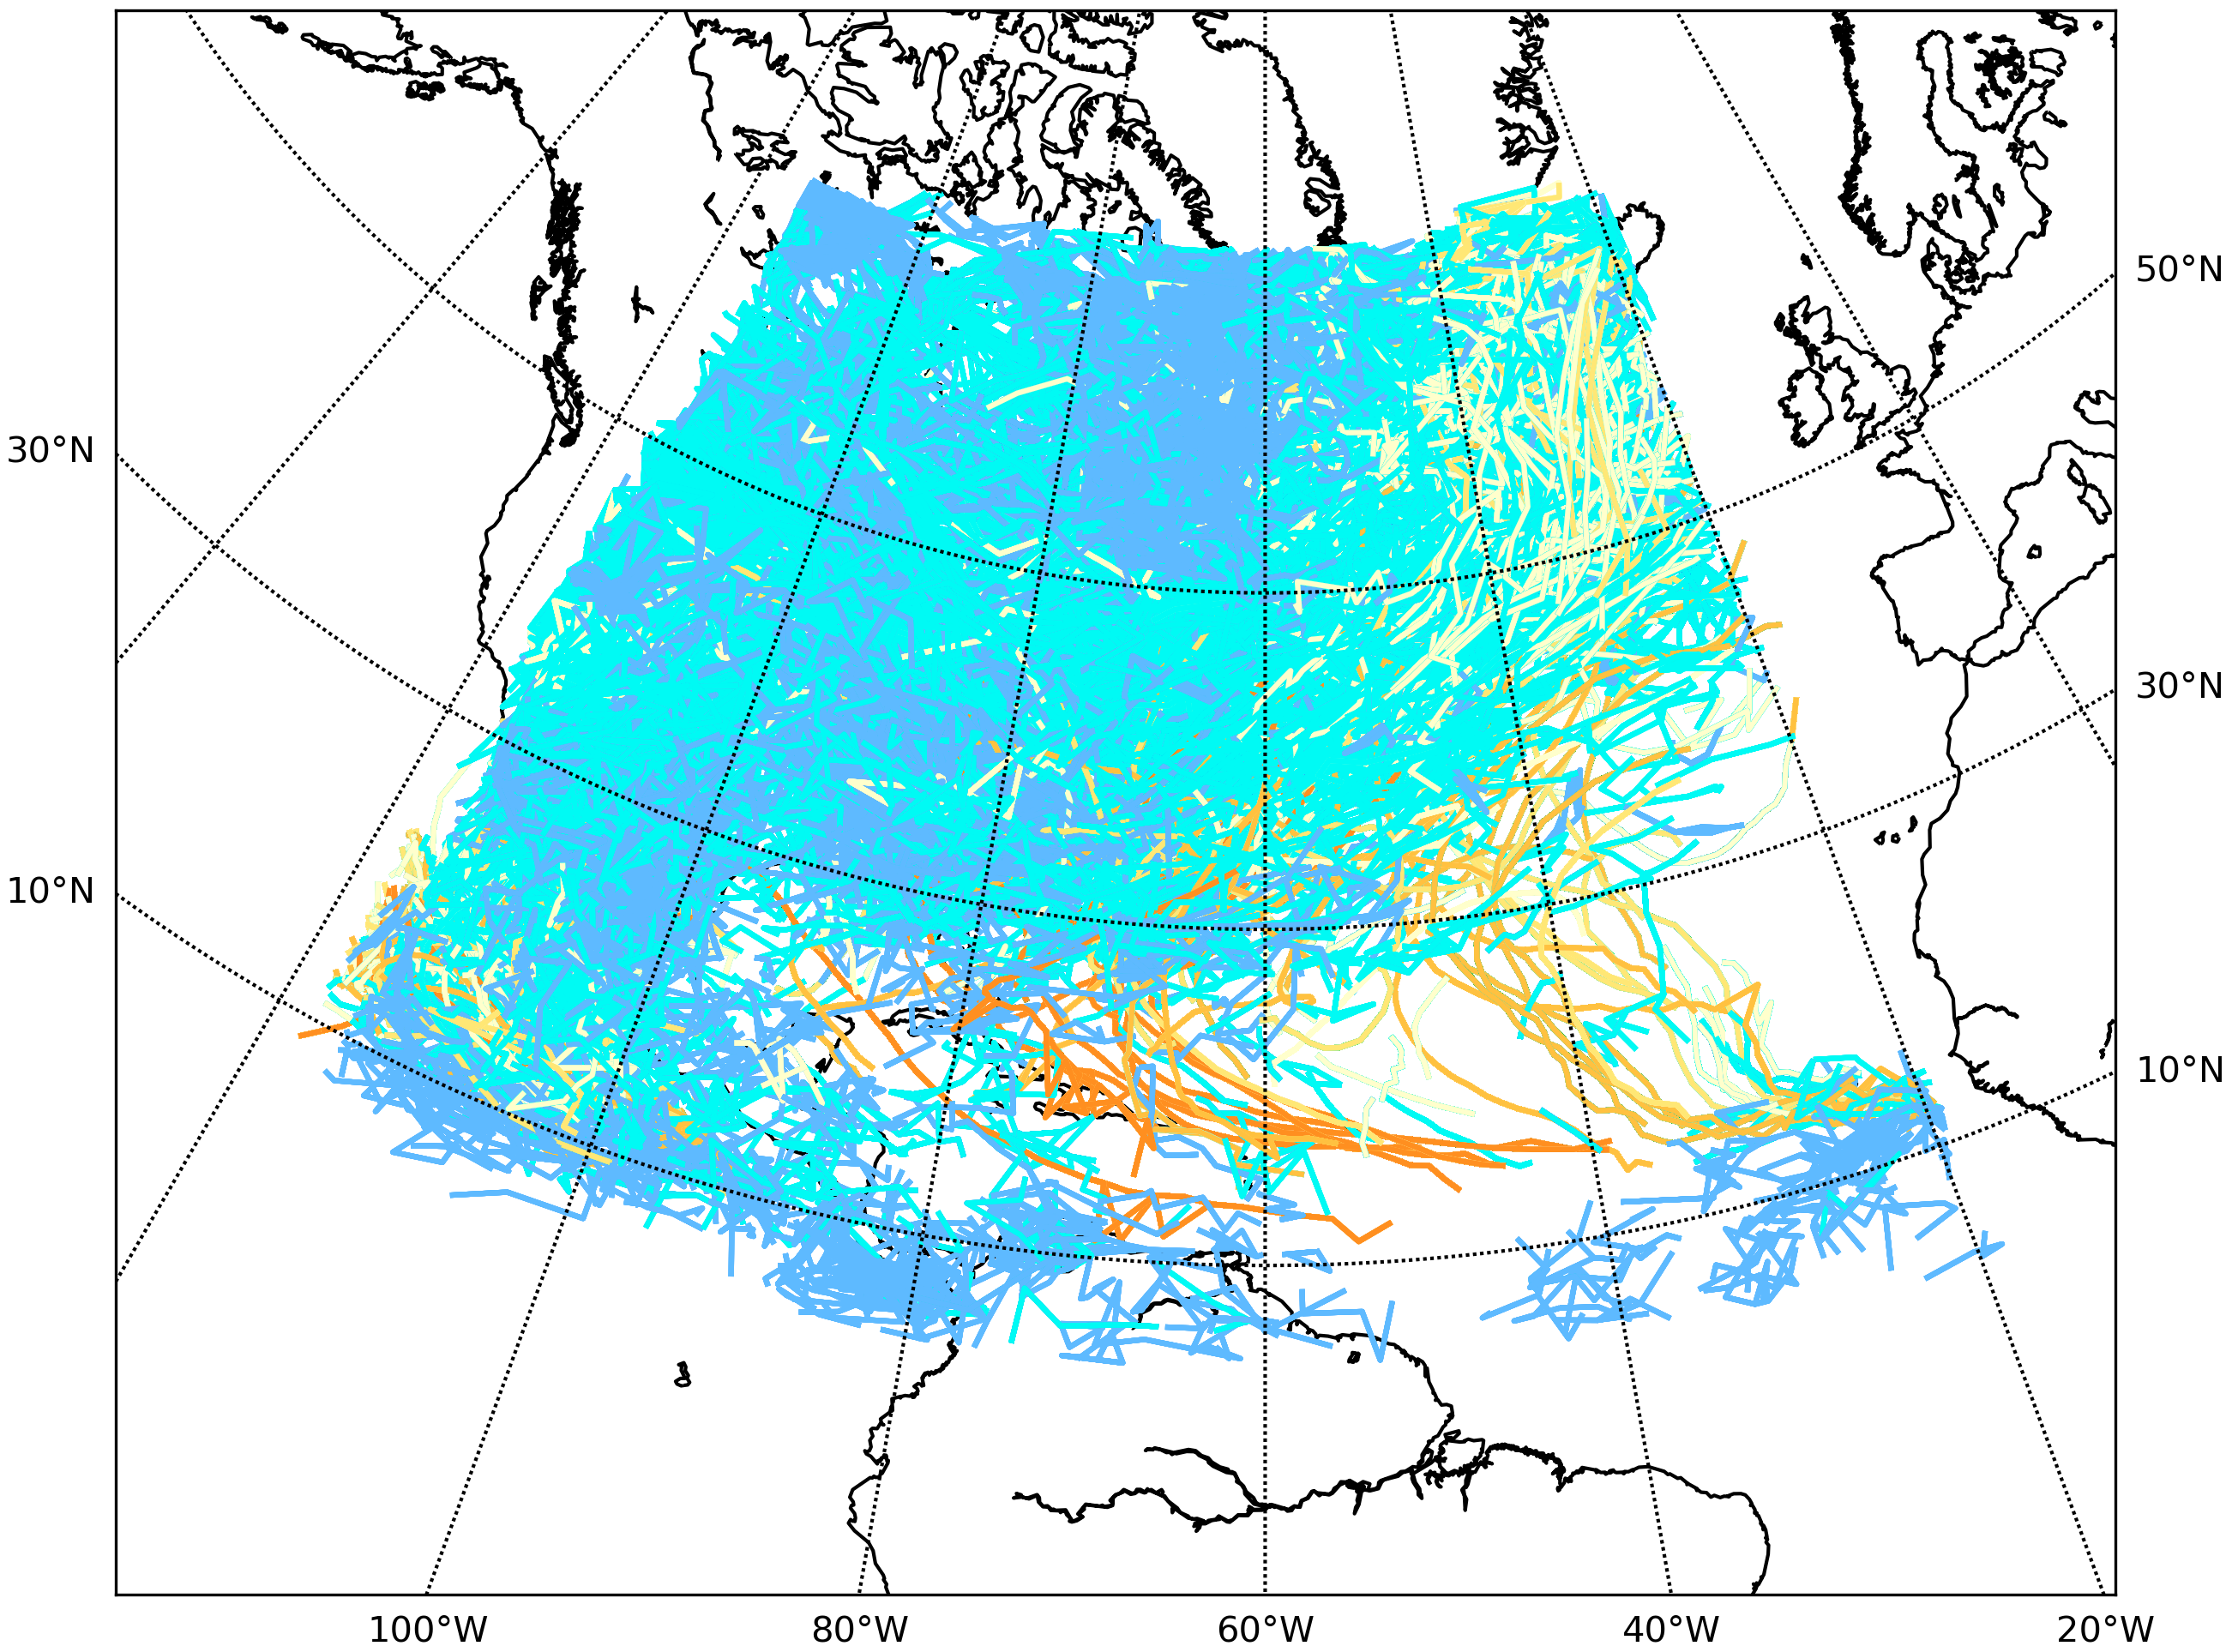
\includegraphics[width = \textwidth]{img/all_tracks.png}
	\end{minipage}
	\hfill
	\begin{minipage}[t]{0.48\textwidth}
		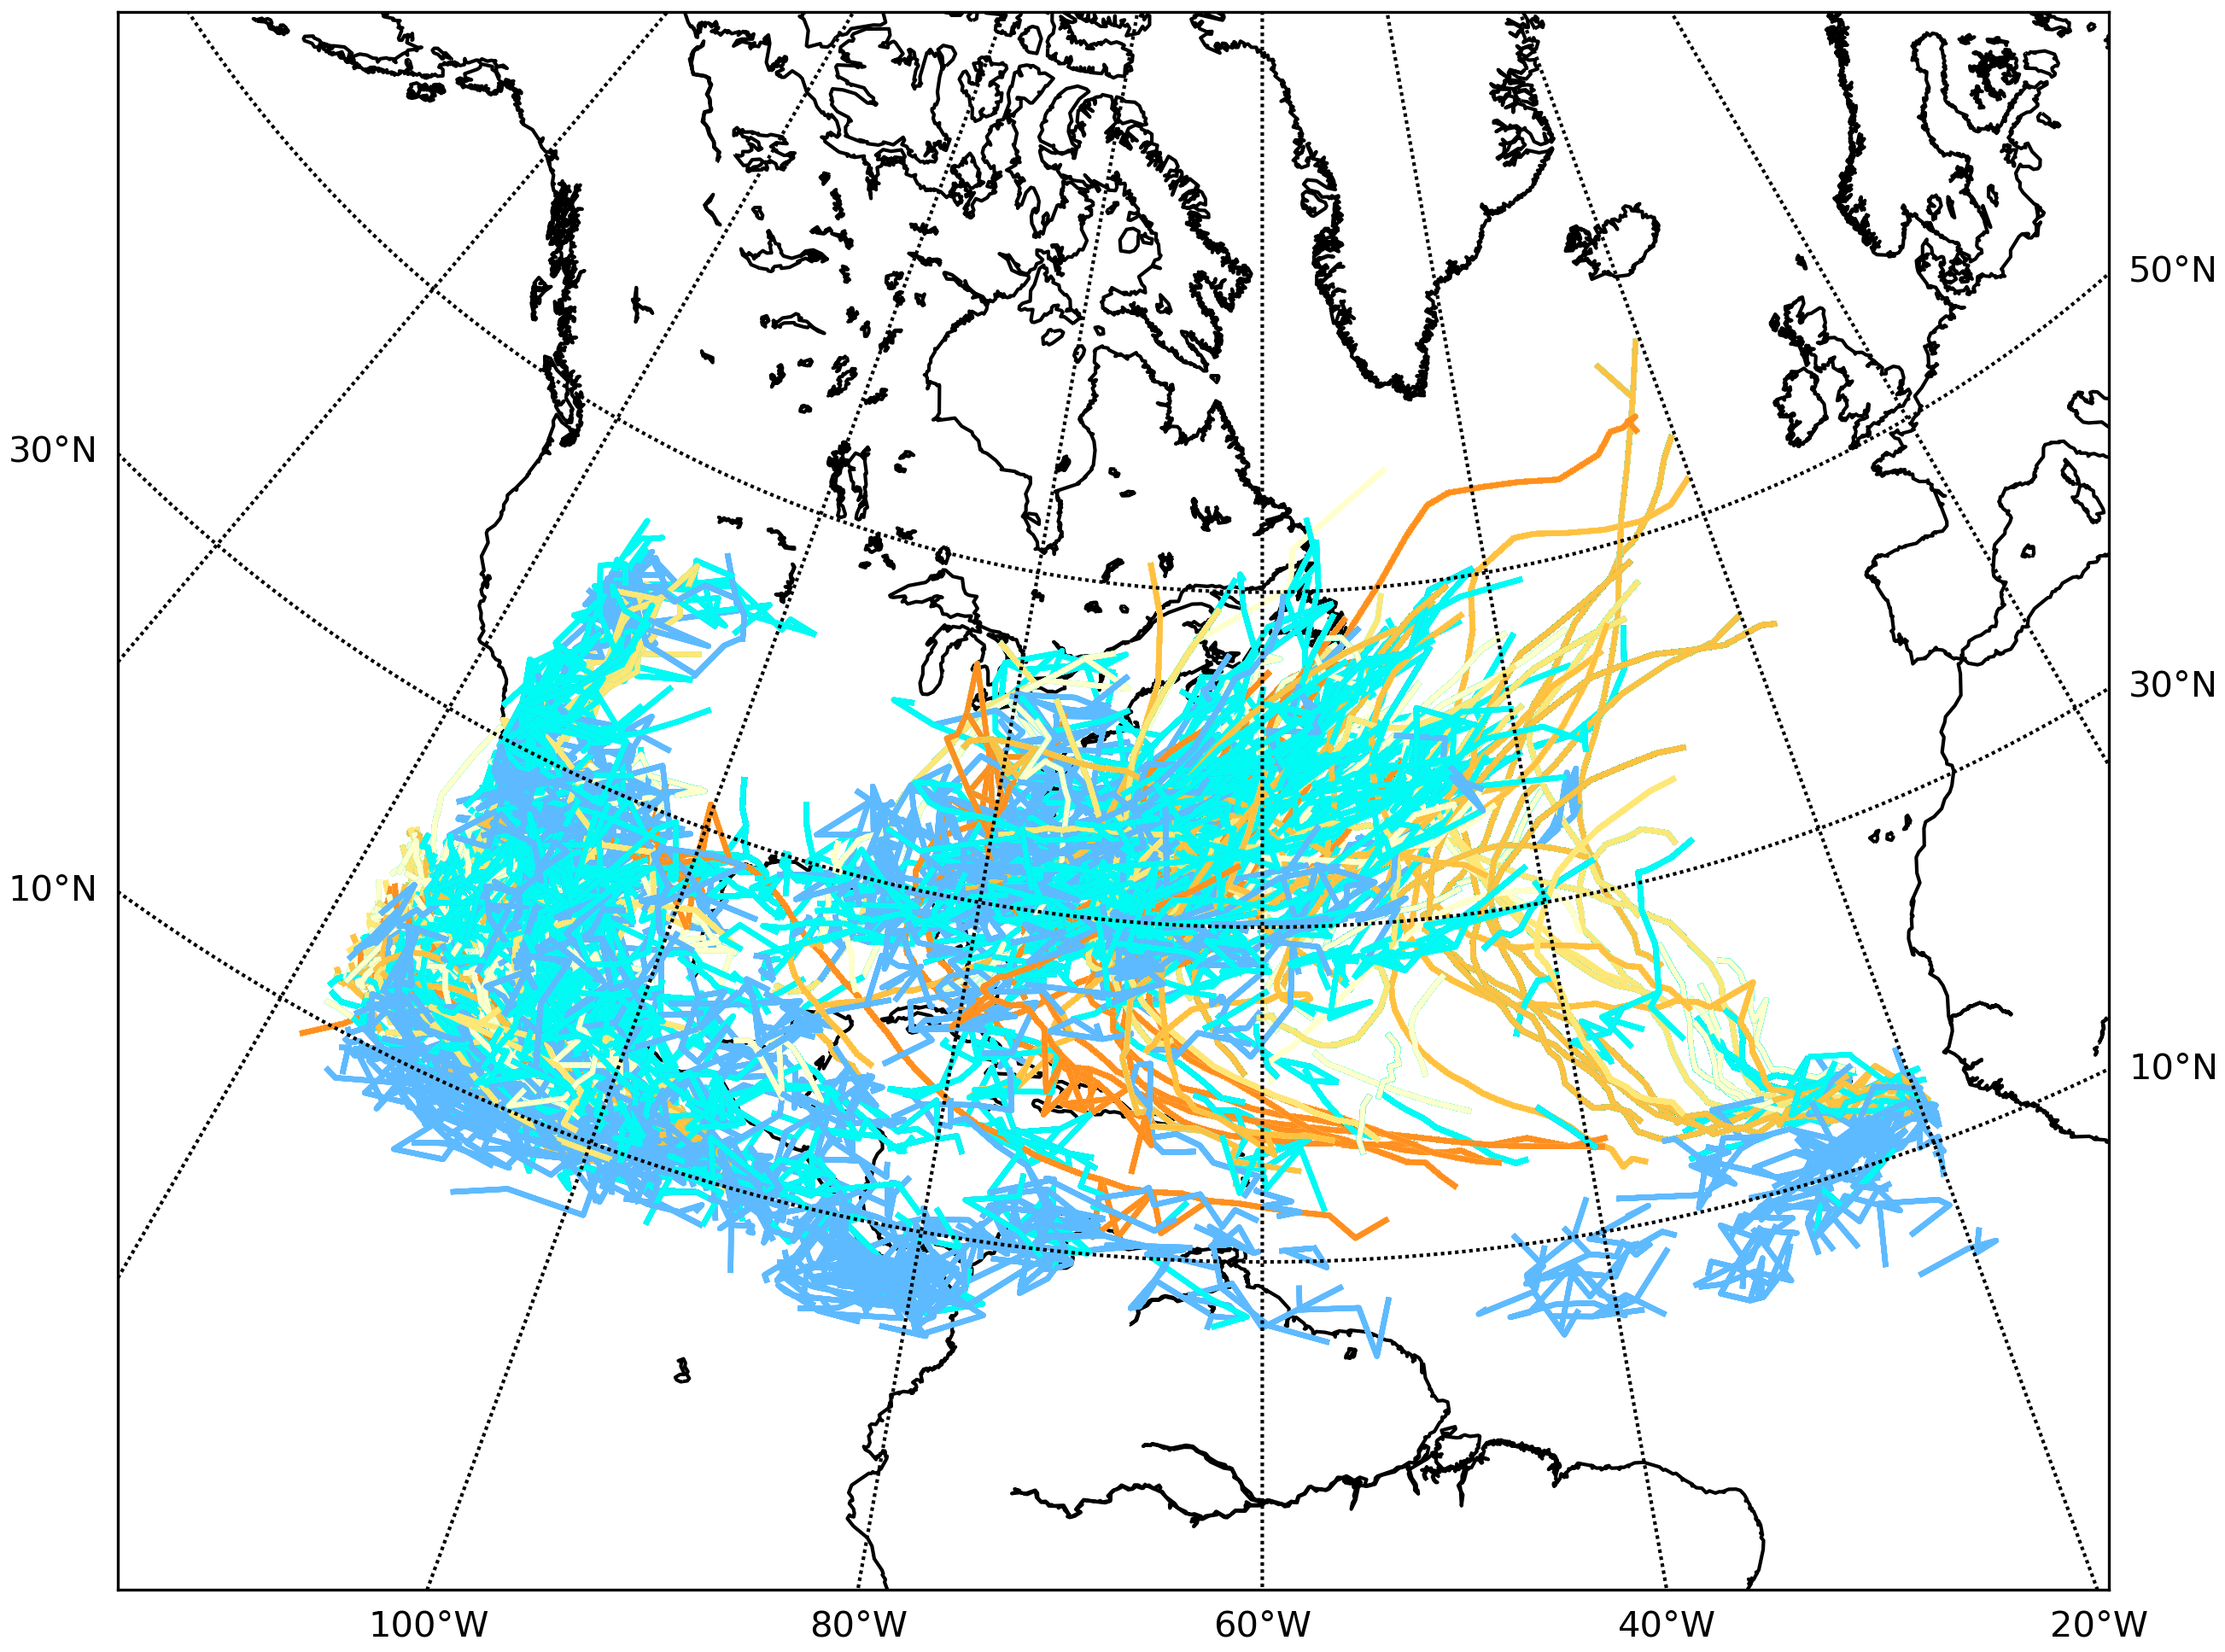
\includegraphics[width = \textwidth]{img/all_tracks_sst.png}
	\end{minipage}
	\caption{Comparison of all tracks without and with the SST criterion on the left and right}
	\label{fig:sst-effect}
\end{figure}
\subsection{Analysis of variation of parameters}
the following comparisons were performed
\cleardoublepage
\chapter{Results}\label{sec:results}

\section{Filtering out noise}\label{sec:noise}
After the tracking and stitching steps are completed, the algorithm results can
still be improved by filtering the results. A large improvement was
achieved by requiring a certain sea surface temperature at TC genesis.
\subsection*{Sea Surface Temperature Criterion}
As outlined in Sec.~\ref{sec:physics} the TCs need warm ocean water as an
energy source, especially when they form. It has been shown that the large
majority has a SST over 25.5\degree C \cite{sst-paper}. Therefore it is
expected that no reasonable TCs are filtered out when requiring a genesis SST
of at least 24\degree C. However as can be seen in Fig.~\ref{fig:sst-effect}
a large part of the unwanted tracks in the North of the domain are removed.
% TODO use figures here and in general with reasonable and elaborated parameters only
\begin{figure}[ht]
	\begin{minipage}[t]{0.48\textwidth}
		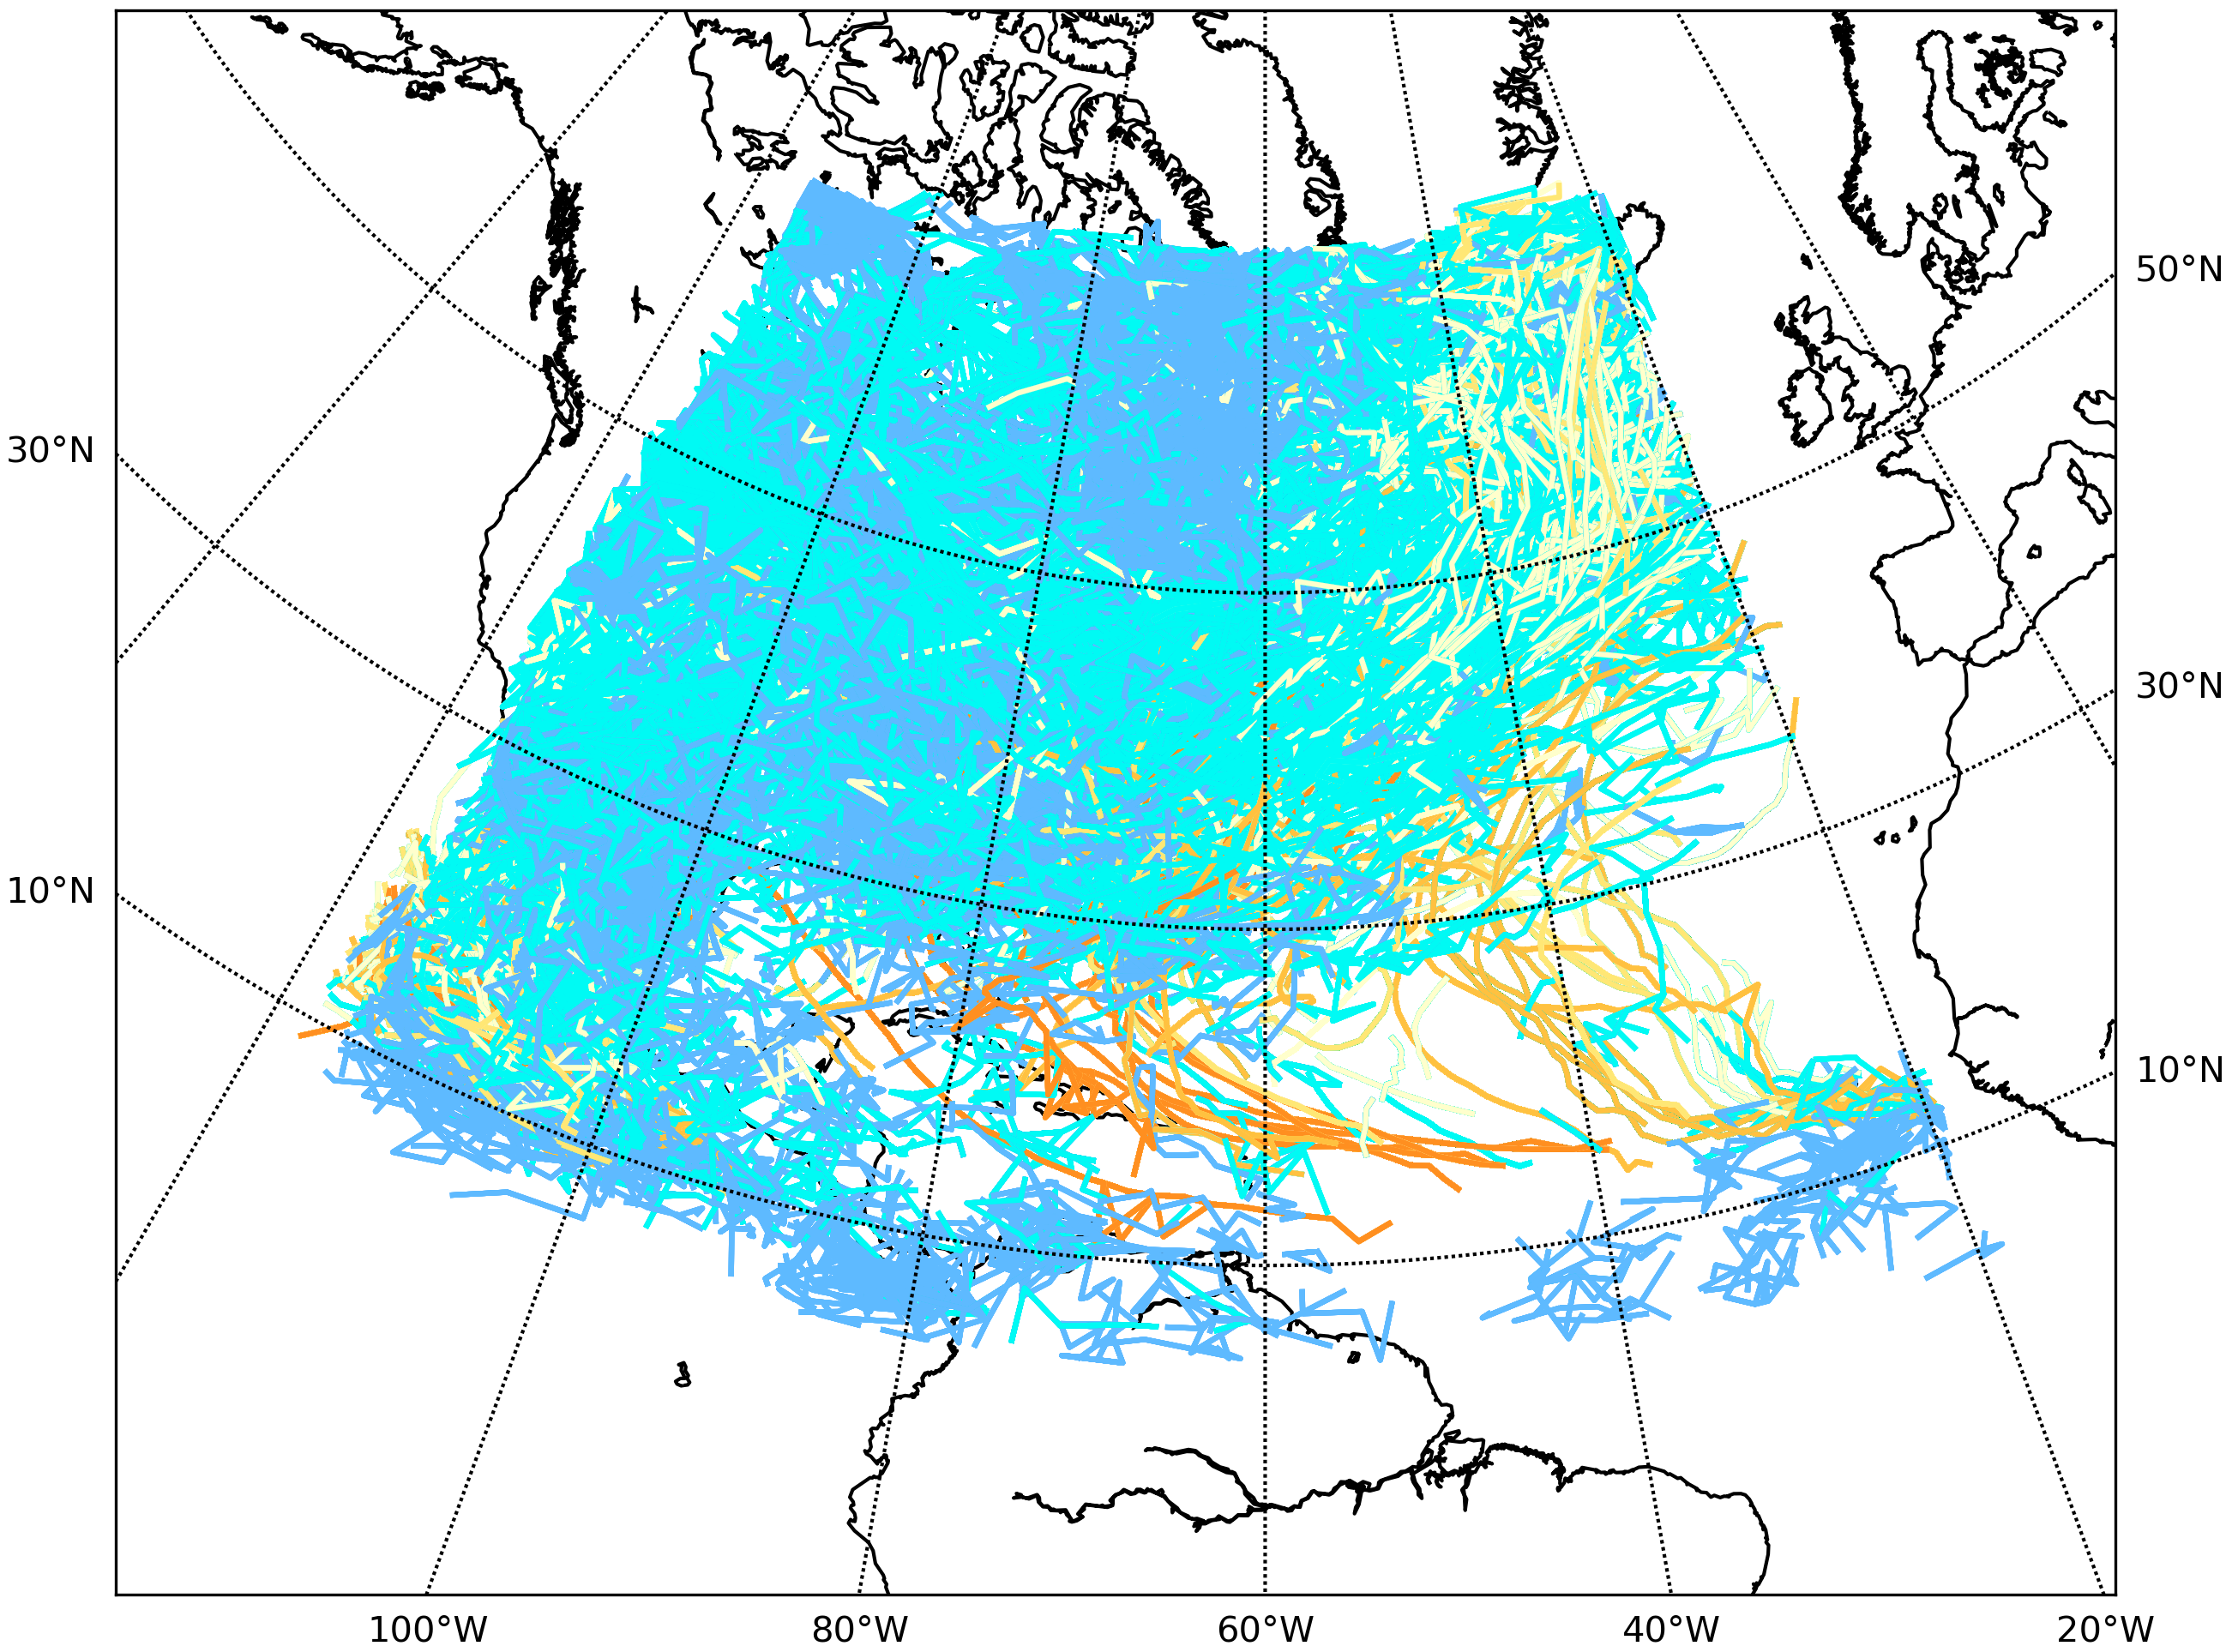
\includegraphics[width = \textwidth]{img/all_tracks.png}
	\end{minipage}
	\hfill
	\begin{minipage}[t]{0.48\textwidth}
		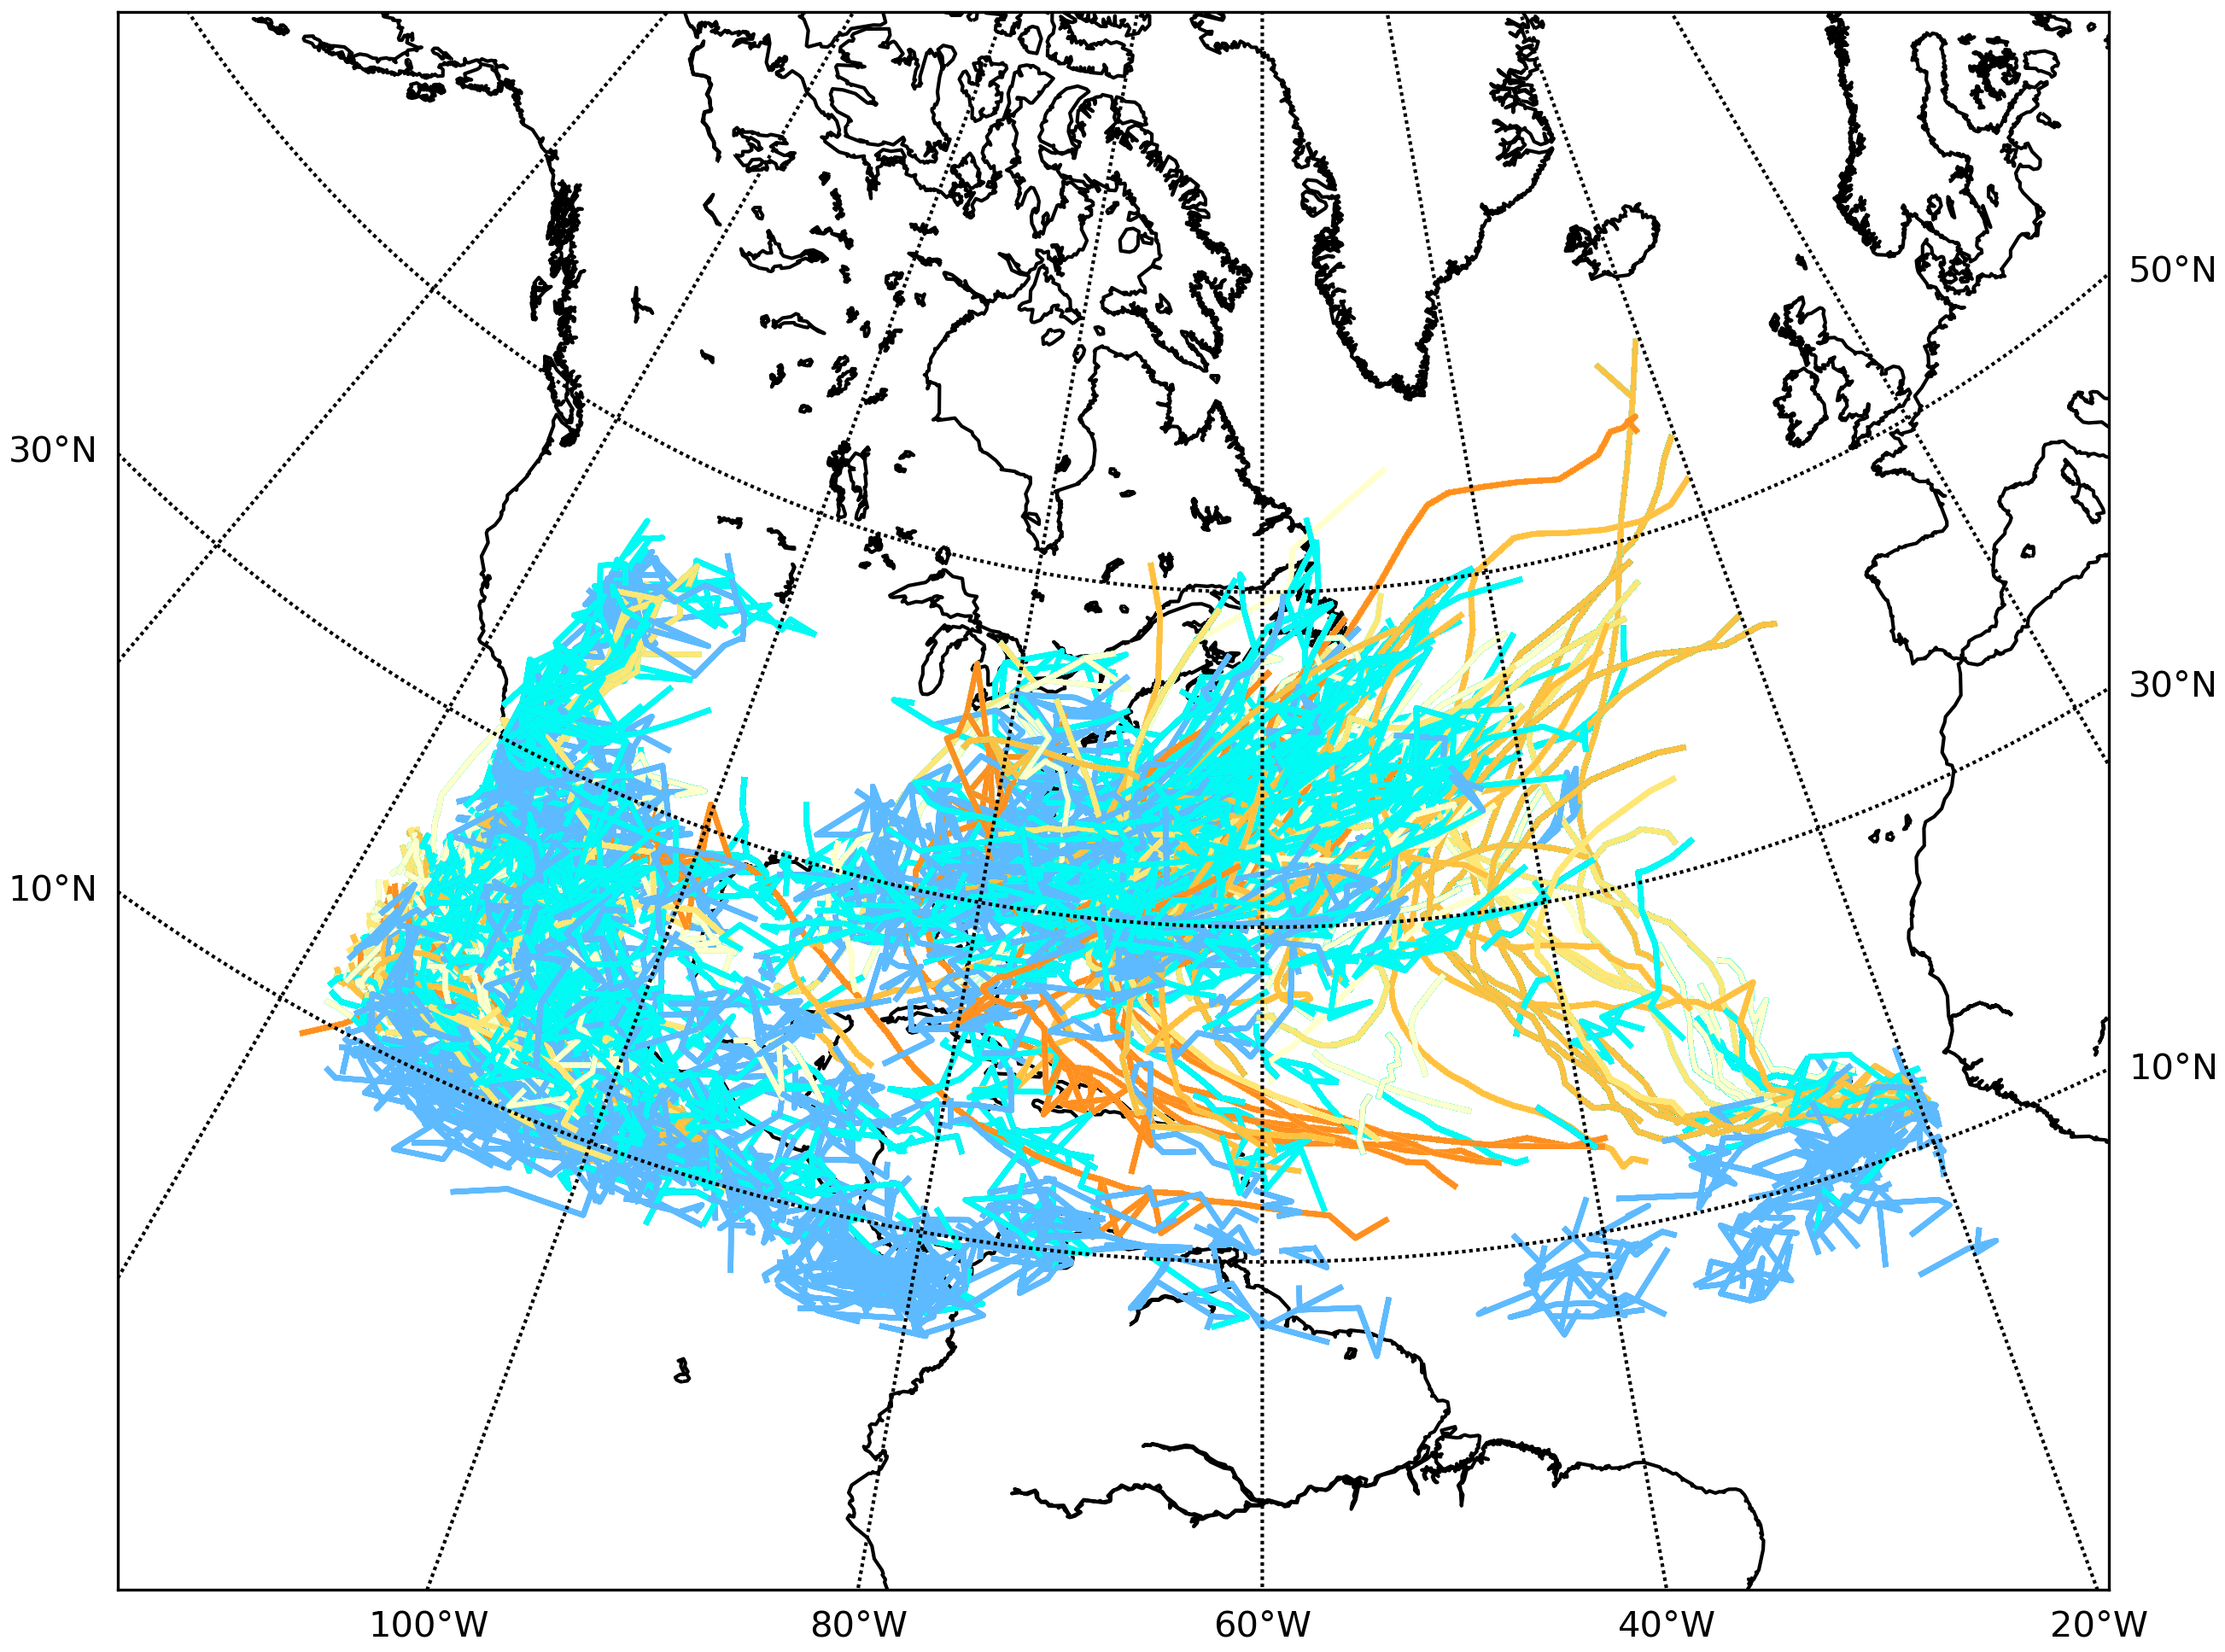
\includegraphics[width = \textwidth]{img/all_tracks_sst.png}
	\end{minipage}
	\caption{Comparison of all tracks without and with the SST criterion on the left and right}
	\label{fig:sst-effect}
\end{figure}

\subsection*{Analysing geographically unreasonable tracks}
Even with the application of the SST-criterion, unreasonable TC tracks remain. For instance the tracks over Wyoming shown in Fig.~\ref{fig:rogue-tracks} should not be so frequent. To determine the parameters responsible for this, the 20 parameter combinations that account for the large majority of these, share the common feature that they all corresponded to the same weak warm core criterion. They had a \textbf{temdif} of \unit[0.5]{\degree C} and a \textbf{temdis} of \unit[400]{km}. Therefore if only a very low temperature difference is required for an area that can be larger than smaller sized TCs, low pressure systems that do not correspond to tropical cyclones are tracked. While this may not be surprising, it does emphasise the importance of a well trimmed warm core criterion.
\begin{figure}[ht]
	\centering
	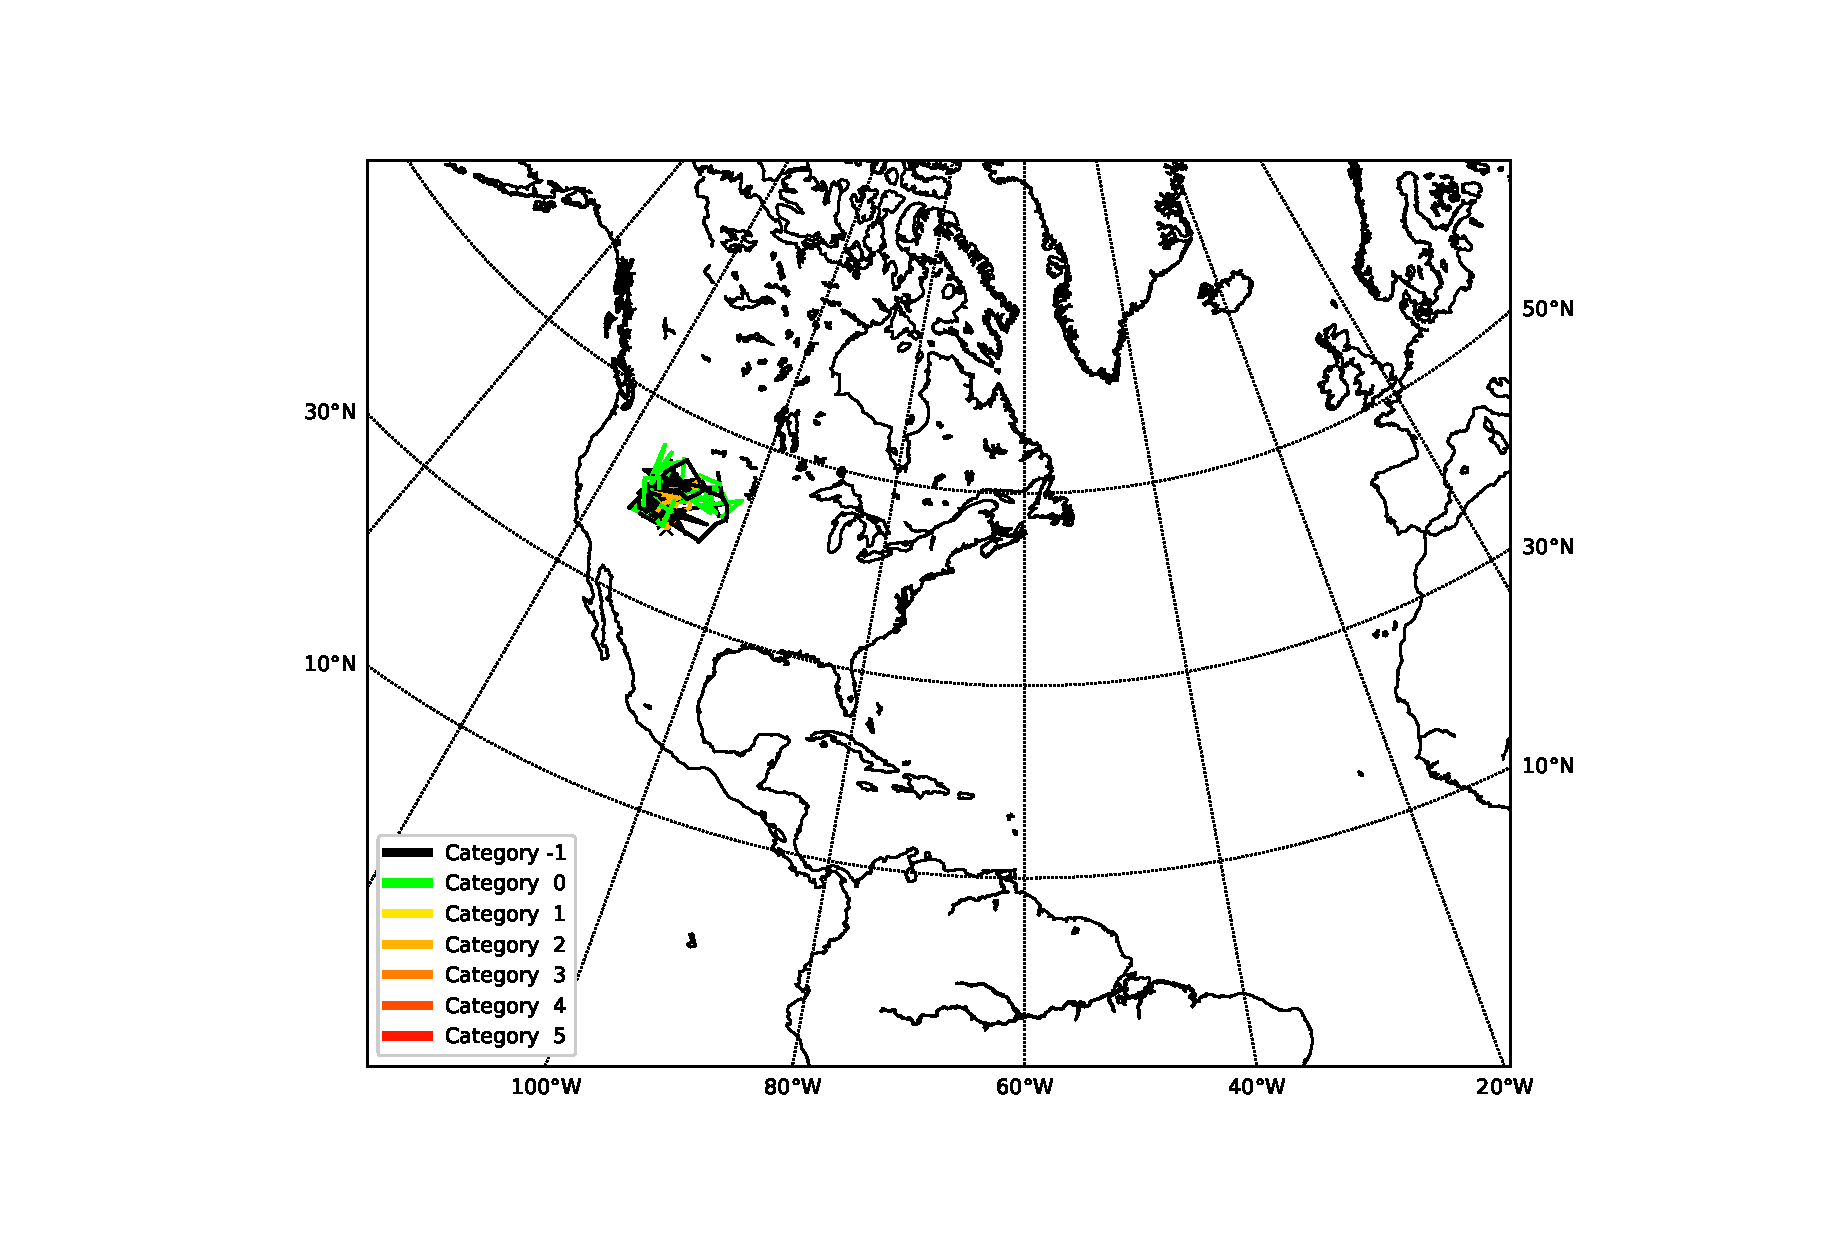
\includegraphics[width=0.7\textwidth]{img/rogue_tracks.eps}
	\caption{Set of unreasonable tracks over Wyoming and the surrounding states}
	\label{fig:rogue-tracks}
\end{figure}
\section{Validating Results}
In Sec.~\ref{sec:noise} it was found that with a sufficiently strong warm core condition the tracks appear in reasonable areas. Before comparing the algorithm output for different parameter combinations, it still remains to be shown that the produced tracks actually follow TCs and not other low pressure systems. For that purpose ten different storms were randomly chosen. For these storms the radial, tangential and vertical wind and the sea level pressure were visualised in the azimuthal mean. It was found that all storms qualitatively exhibit the physically expected structure that was described in Sec.~\ref{sec:physics}. The resulting plots for a representative storm can be seen in Fig.~\ref{fig:azimean}.

\begin{figure}[b]
\centering
\begin{subfigure}{.5\linewidth}
    \centering
    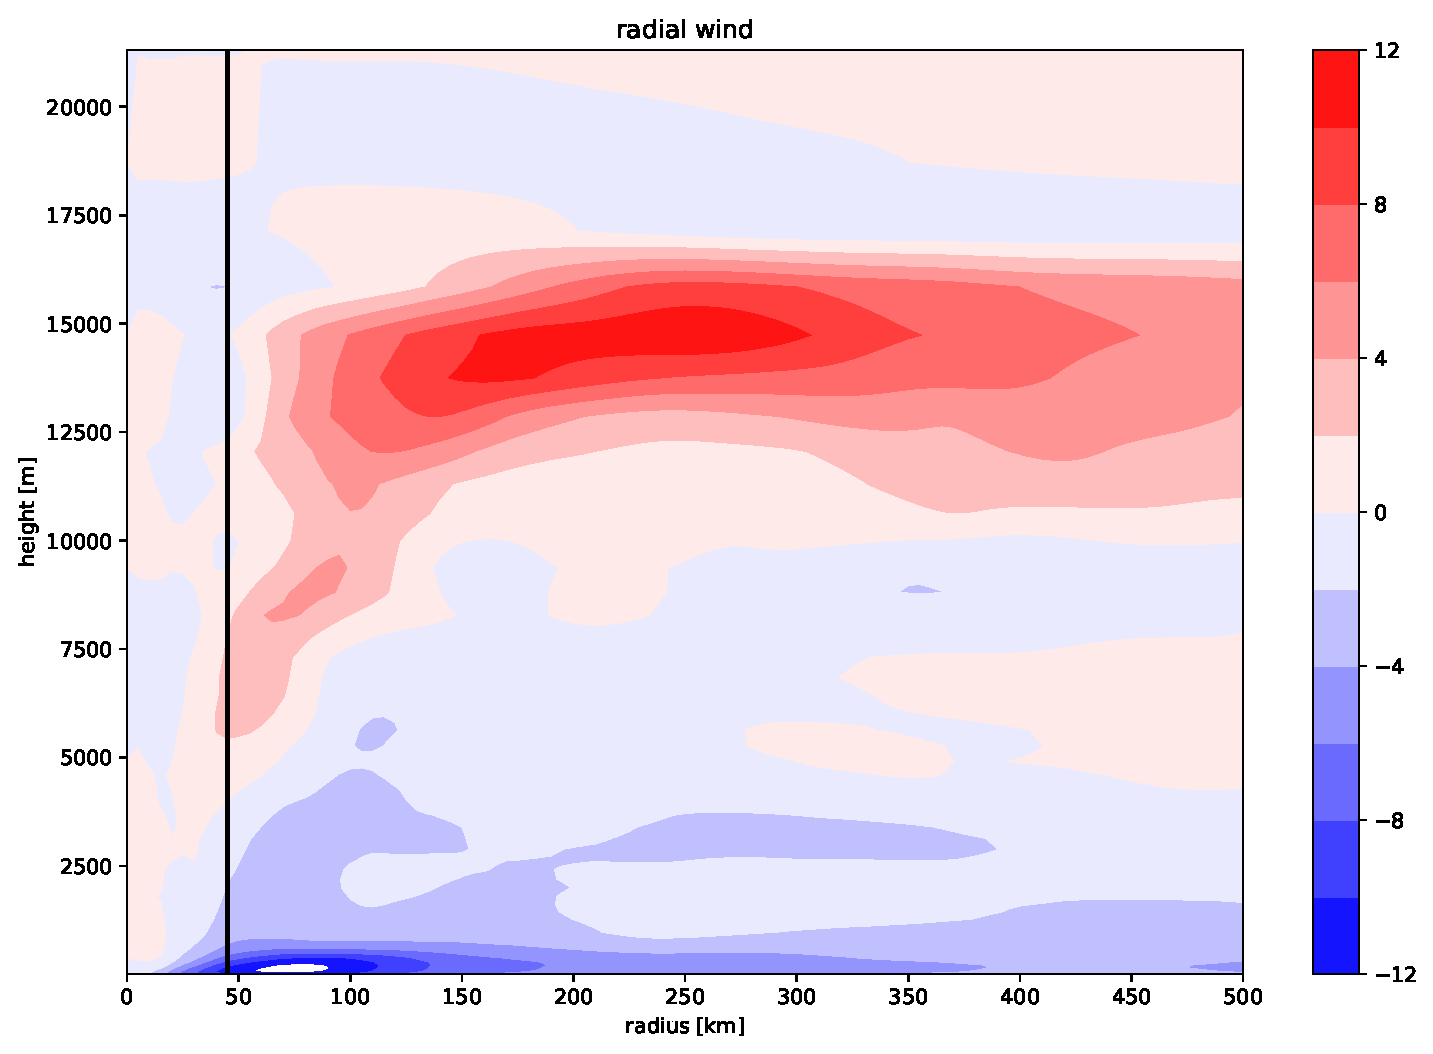
\includegraphics[width=0.75\linewidth]{img/tight09279566radwind20130706T120000Z.eps}
\end{subfigure}%
\begin{subfigure}{.5\linewidth}
    \centering
    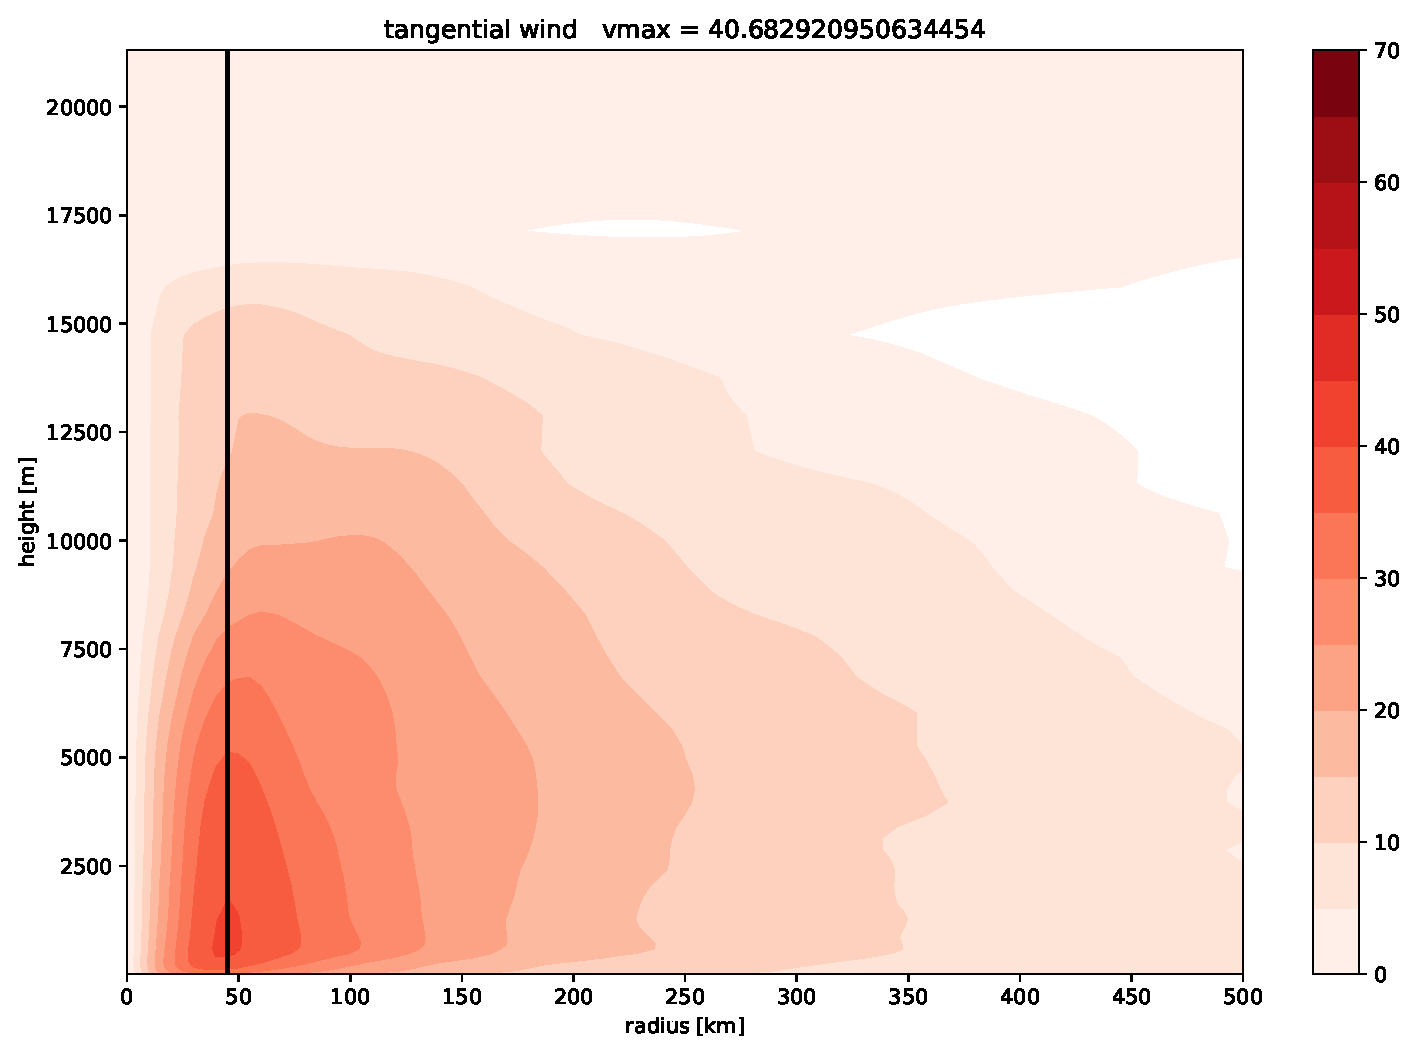
\includegraphics[width=0.75\linewidth]{img/tight09279566tanwind20130706T120000Z.eps}
\end{subfigure}
\begin{subfigure}{.5\linewidth}
    \centering
    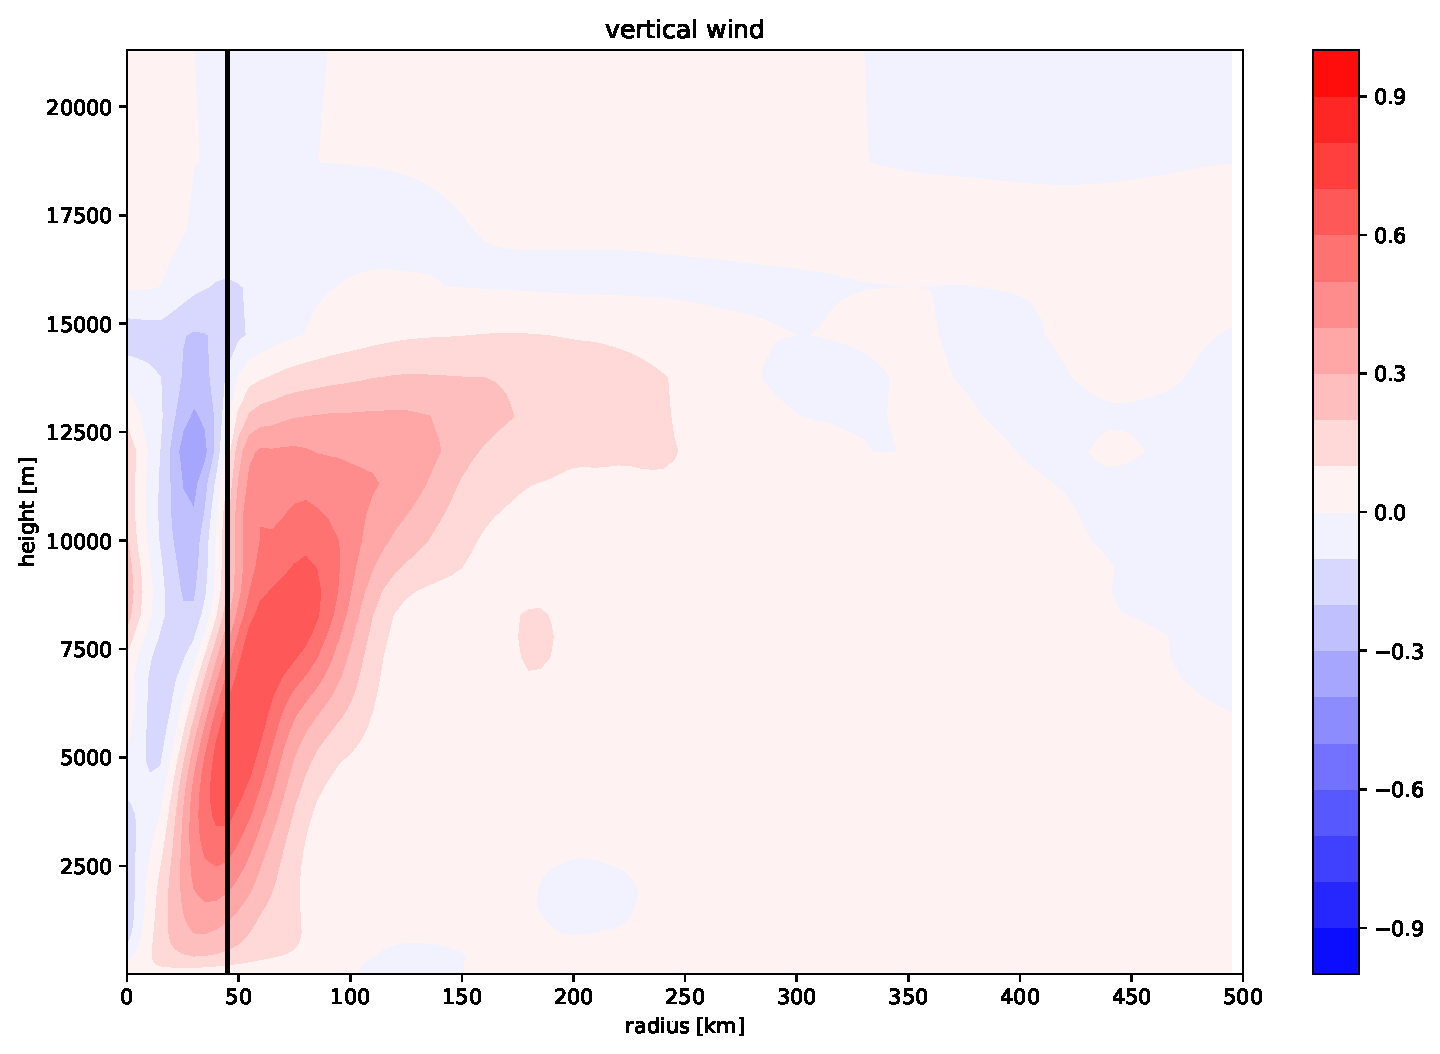
\includegraphics[width=0.75\linewidth]{img/tight09279566verwind20130706T120000Z.eps}
\end{subfigure}%
\begin{subfigure}{.5\linewidth}
    \centering
    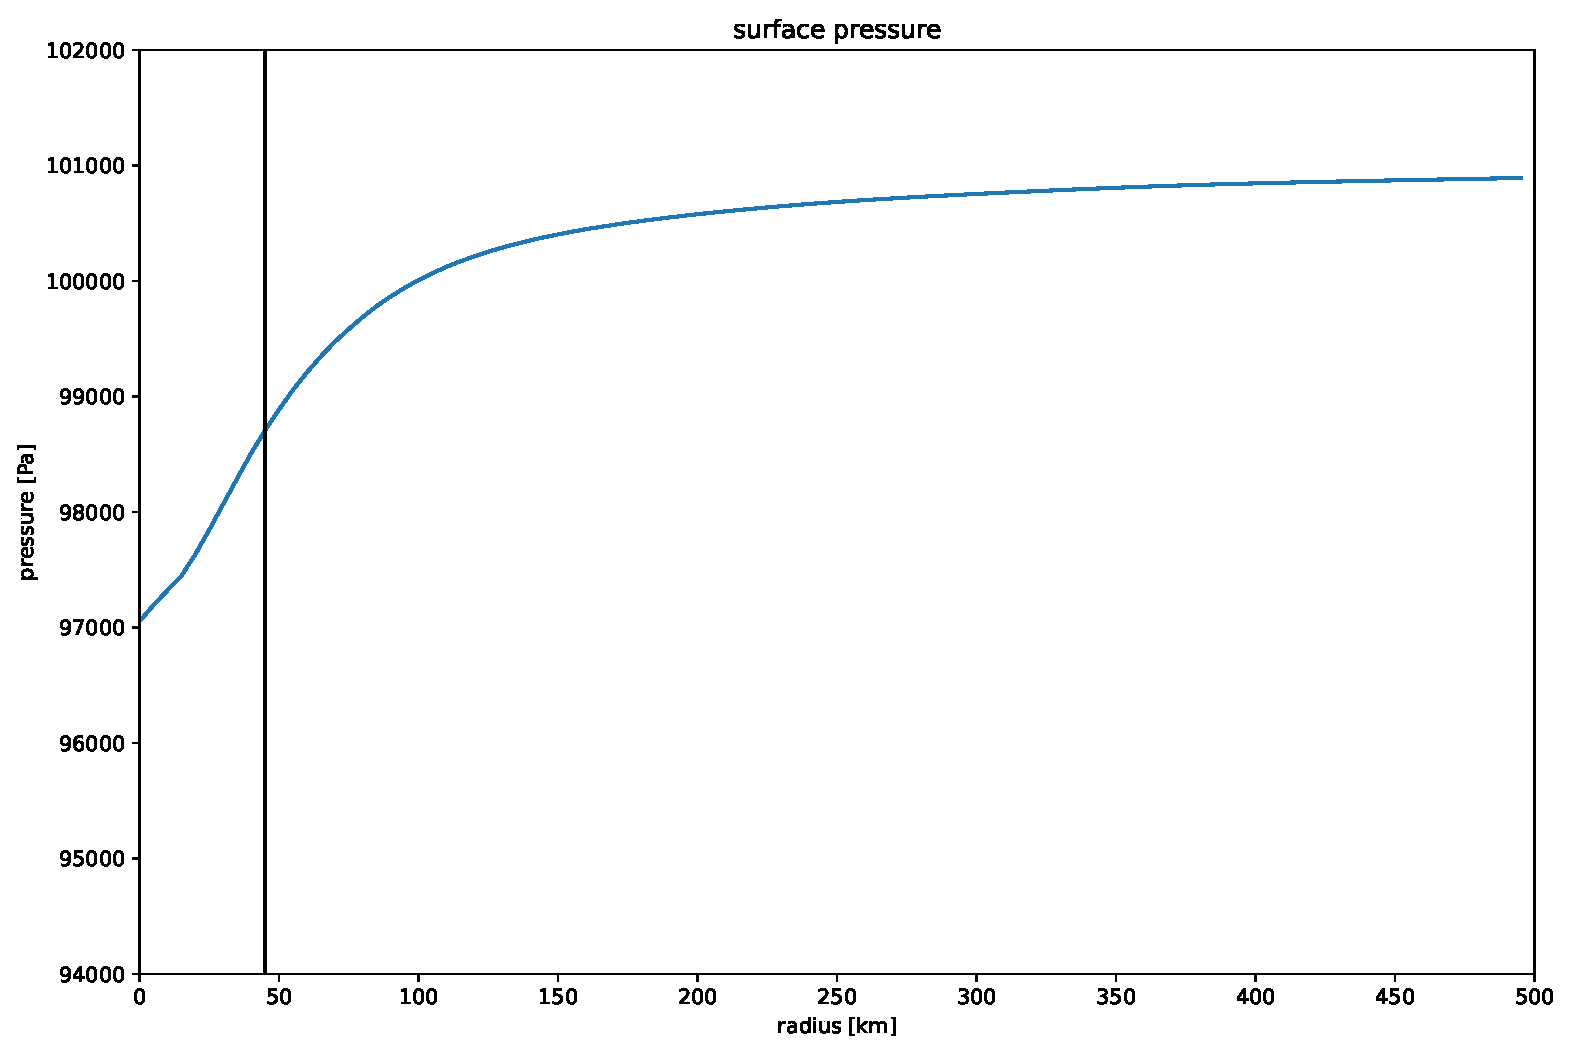
\includegraphics[width=0.75\linewidth]{img/tight09279566pres_msl20130706T120000Z.eps}
\end{subfigure}
\caption[short]{Azimuthal mean plots. From left to right and top to bottom: radial wind, tangential wind, vertical wind and sea level pressure.}
\end{figure}


\section{Variation of the Warm Core Criterion strength}
With the aim of understanding the impact of different warm core criteria strengths, the resulting cyclone distributions for a range of different \textbf{temdif}s were compared. As can be seen in Fig.~\ref{fig:temdif-analysis}, a weaker warm core criterion leads to a distribution with more lower intensity storms. When comparing with the absolute counts it can be seen that this is the result from weaker storms being tracked for lower \textbf{temdif}s. Logically for TCs of category 2 and upwards, no difference in the counts is observed. Furthermore for \textbf{temdif}s larger than \unit[1]{K}, no tropical depressions which correspond to category -1 are tracked. It can therefore be concluded that the warm core criterion can be used very efficiently to filter out noise if only strong TCs are of interest.
% TODO create plot that analyses category snapshots for tcs with max cat=2 and above
\begin{figure}[ht]
	\begin{minipage}[t]{0.48\textwidth}
		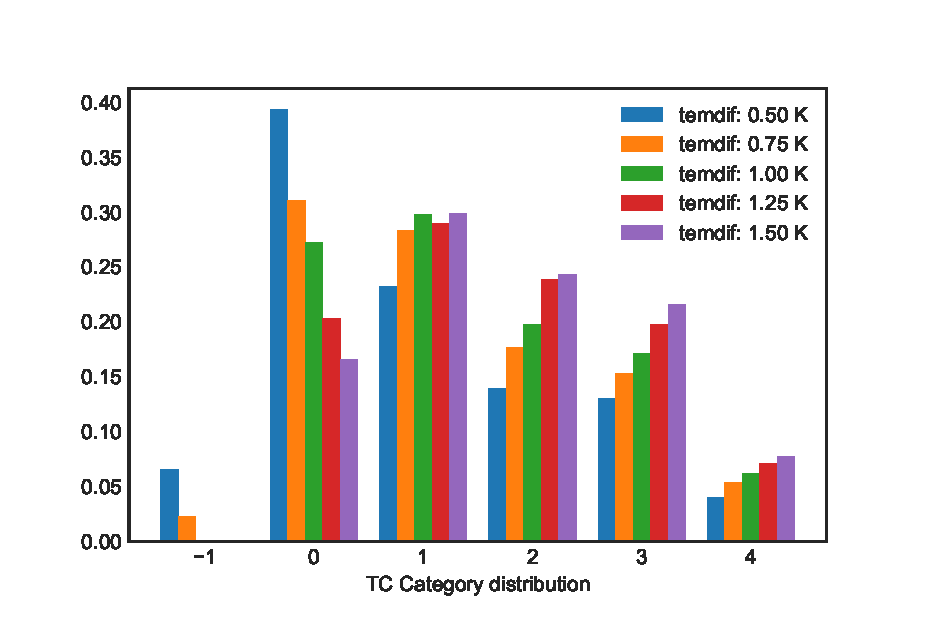
\includegraphics[width = \textwidth]{img/max_cat_distr_temdifs.eps}
	\end{minipage}
	\hfill
	\begin{minipage}[t]{0.48\textwidth}
		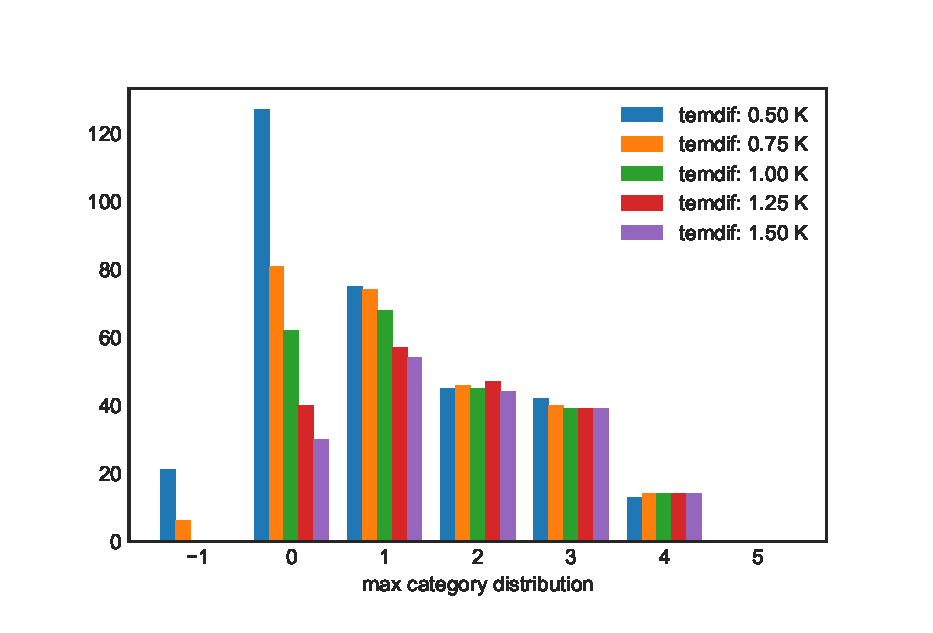
\includegraphics[width = \textwidth]{img/max_cat_counts_temdifs.eps}
	\end{minipage}
	\caption{Maximum TC category histograms for different \textbf{temdif} parameters. Each histogram on the left has unit norm. The right plot shows the absolute counts of TCs. The X-axis describes the TC categories as defined in Tab~\ref{tab:simpson-scale}.}
	\label{fig:temdif-analysis}
\end{figure}


\section{Comparison of the Warm Core Criterion and the Vorticity Threshold}\label{sec:warmcore-var}
In order to compare the importance of the warm core criterion with the vorticity threshold, TCs were tracked with parameter combinations of varying relative strength of the two criteria. To be concrete, all nine combinations of the parameters in Tab.~\ref{tab:vor-tem-comparison} were used.

\begin{table}[ht]
	\centering
	\begin{tabular}{|l|l|l|}
		\hline
		\textbf{parameter} & \textbf{unit} & \textbf{values}  \\ \hline
		slpdis             & m             & 100000           \\
		vormin             & 1/s           & 1e-6, 1e-5, 1e-4 \\
		temdif             & K             & 0.5, 1 ,1.5      \\
		temdis             & m             & 200000           \\ \hline
	\end{tabular}
	\caption{Parameter combinations used for the comparison}
	\label{tab:vor-tem-comparison}
\end{table}
% TODO really think about this and the max category influence of vorticity ask Bernhard
It was expected that the vorticity threshold should influence the distribution of tracked TCs only if a weak warm core criterion is applied. However, as can be seen in Fig.~\ref{fig:temdif-vormin-comp}, even with a very weak warm core criterion does the vorticity threshold not influence the storm intensity distributions. A comparison for different values of \textbf{temdif} and an analysis of the impact of the vorticity criterion on the storm lifetime, can be found in the Appendix.

\begin{figure}[ht]
	\centering
	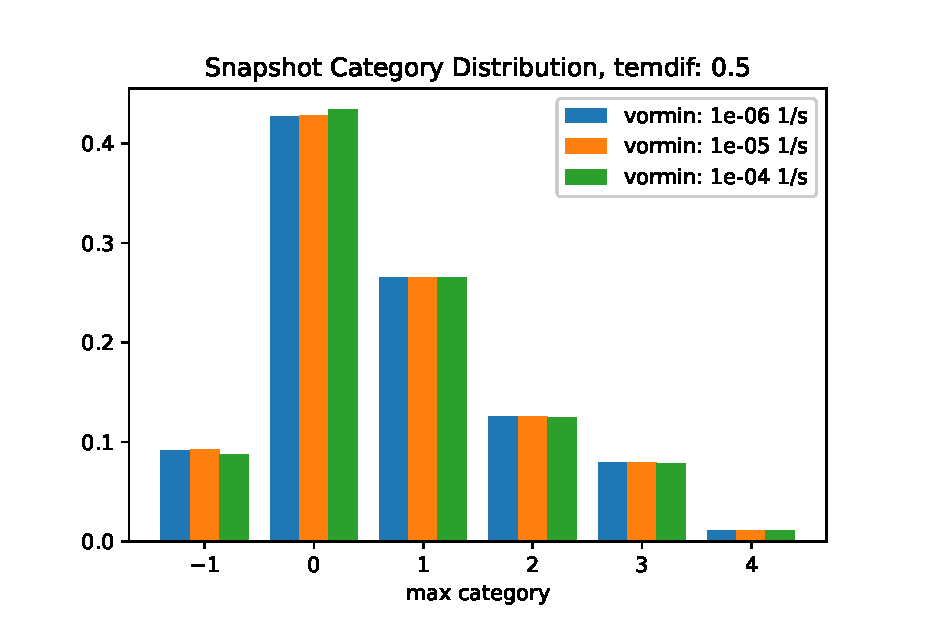
\includegraphics[width=0.7\textwidth]{img/curr_category_vortem05.eps}
	\caption{Snapshot category distribution for a weak warm core criterion and several vorticity thresholds}
	\label{fig:temdif-vormin-comp}
\end{figure}

\section{TC Genesis regions}
A direct consequence of the observations from Sec.~\ref{sec:warmcore-var} is that with a weaker warm core criterion the TCs can be found already when they have not had much time to intensify. This is relevant since from best track data it is expected that most TCs form in the main development region (MDR) which lies roughly between 10 -- 20 degree North and 20 -- 80 degree West. However, when checking the genesis spots and density in Fig.~\ref{fig:genesis-temdif1}, it can be seen that the MDR is not quite satisfied. When using a weaker warm core criterion 
\begin{figure}[ht]
	\centering
	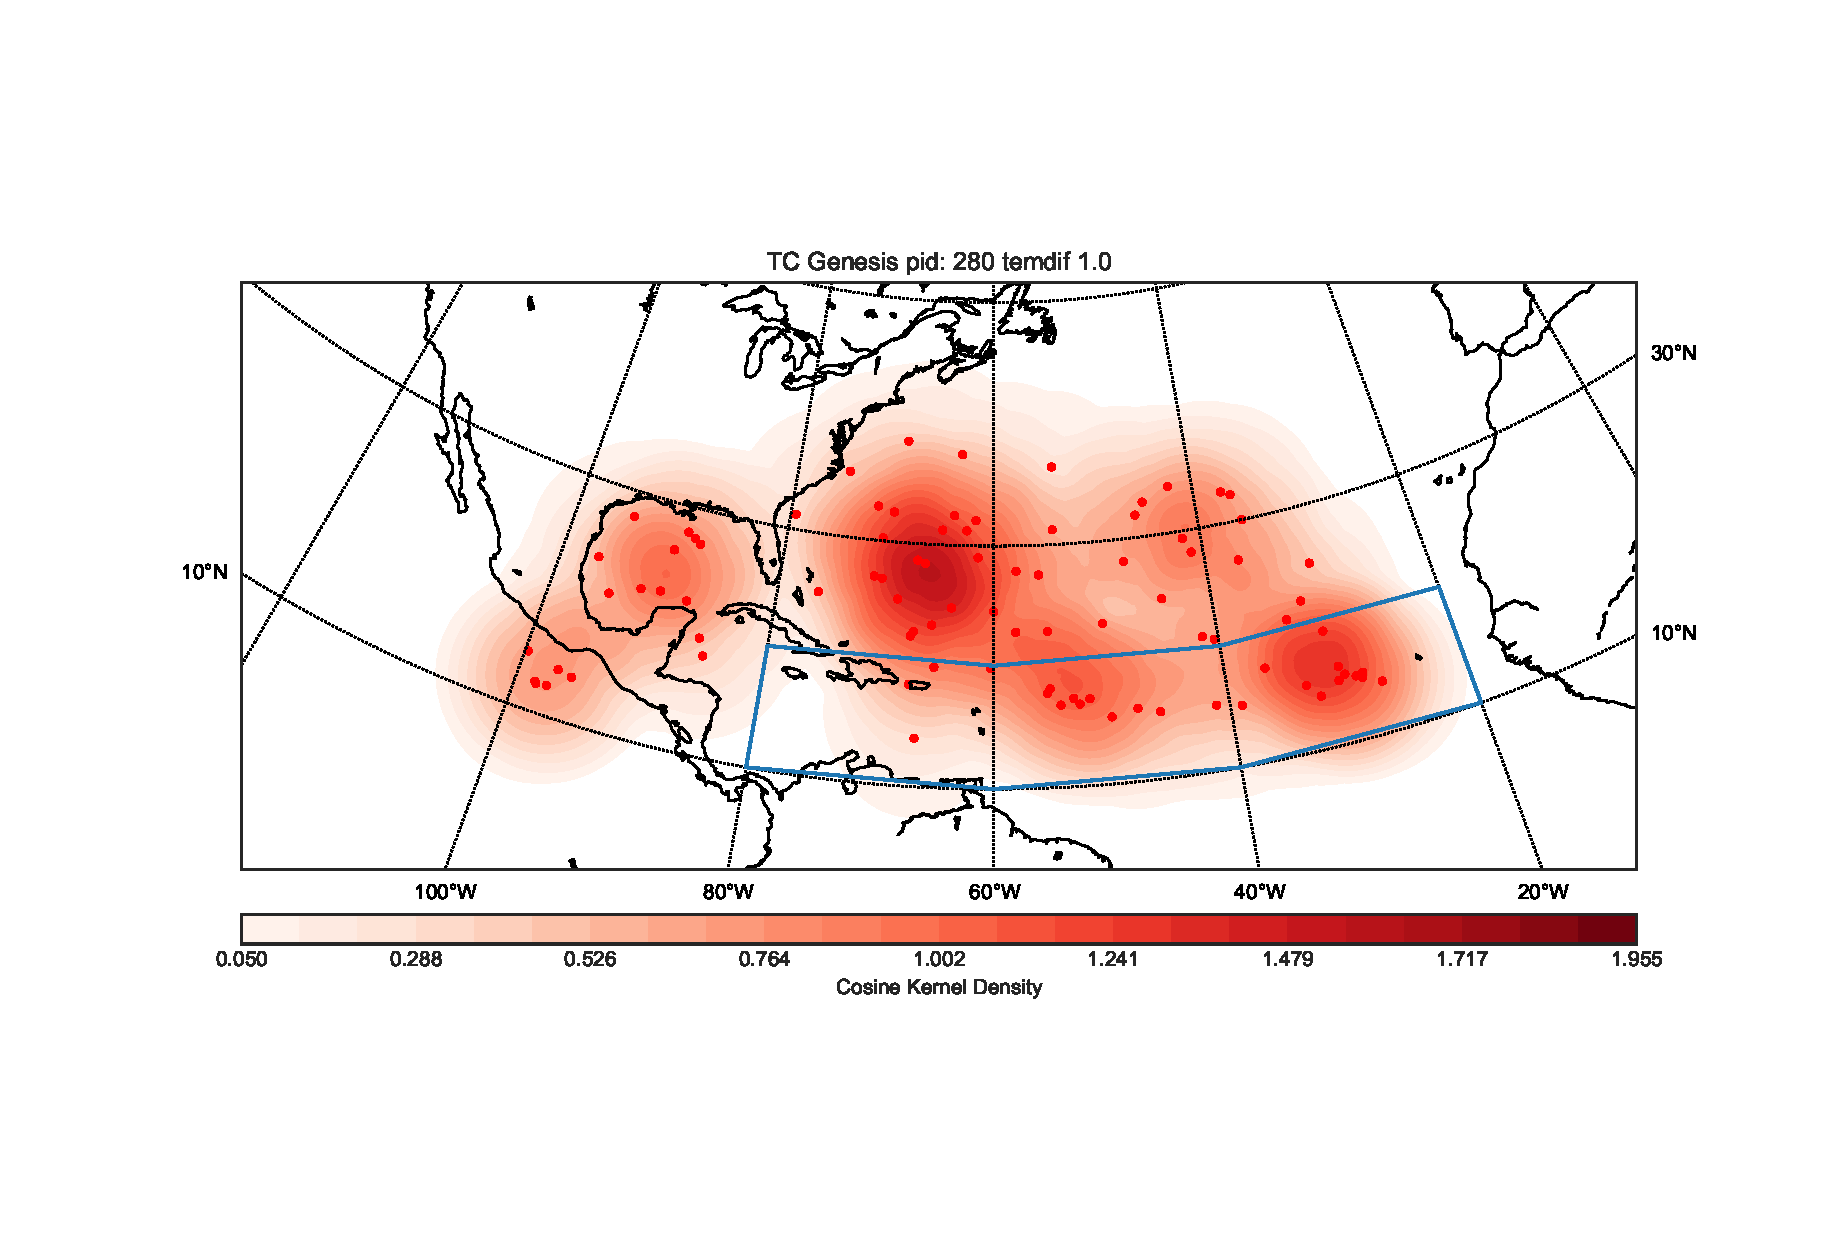
\includegraphics[width=0.7\textwidth]{img/genesis_plot_temdif1.eps}
	\caption{Genesis spots and density for a specific parameter combination.}
	\label{fig:genesis-temdif1}
\end{figure}
%TODO check counts instead of density
%\section{Importance of different criteria}

%\begin{enumerate}
%    \item which criteria have a large impact on the found tcs
%    \item what are interesting thresholds
%    \item Include fascinating plots
%\end{enumerate}


%\section{Recommended parameter combination}
%\begin{enumerate}
%    \item propose combination of parameters for robust search
%\end{enumerate}

\cleardoublepage
\chapter{Conclusion}\label{sec:conclusion}
This project significantly improved the speed and efficiency of a TC tracking algorithm. This speedup enables a comprehensive analysis of different parameter threshold settings. An exploratory data analysis revealed interesting aspects of the different tracking criteria as outlined before. The capability to quickly try different parameter combinations and the already produced tracking data empowers a wide range of further analysis steps. One idea would be to try to reduce \newline
Furthermore the combination of several criteria is a perspective for continuing research and development. It would for instance be interesting to only track storms that satisfy the at least two of three given parameter threshold combinations.

\begin{enumerate}
    \item repeat most important findings
    \item mention further algorithm ideas
    \item suggest more elaborate parallelization with eg dask for improved simulation data reading
\end{enumerate}
\cleardoublepage
% \input{}
% \cleardoublepage
% \input{}
% \cleardoublepage
% ...

% Appendix______________________________________________________________________
\appendix
%\chapter{Something}\label{sec:something}

%Blah, blah \dots

% \cleardoublepage


\chapter{Additional TC Genesis Plots}\label{sec:genesis-appendix}

\begin{figure}[ht]
	\centering
	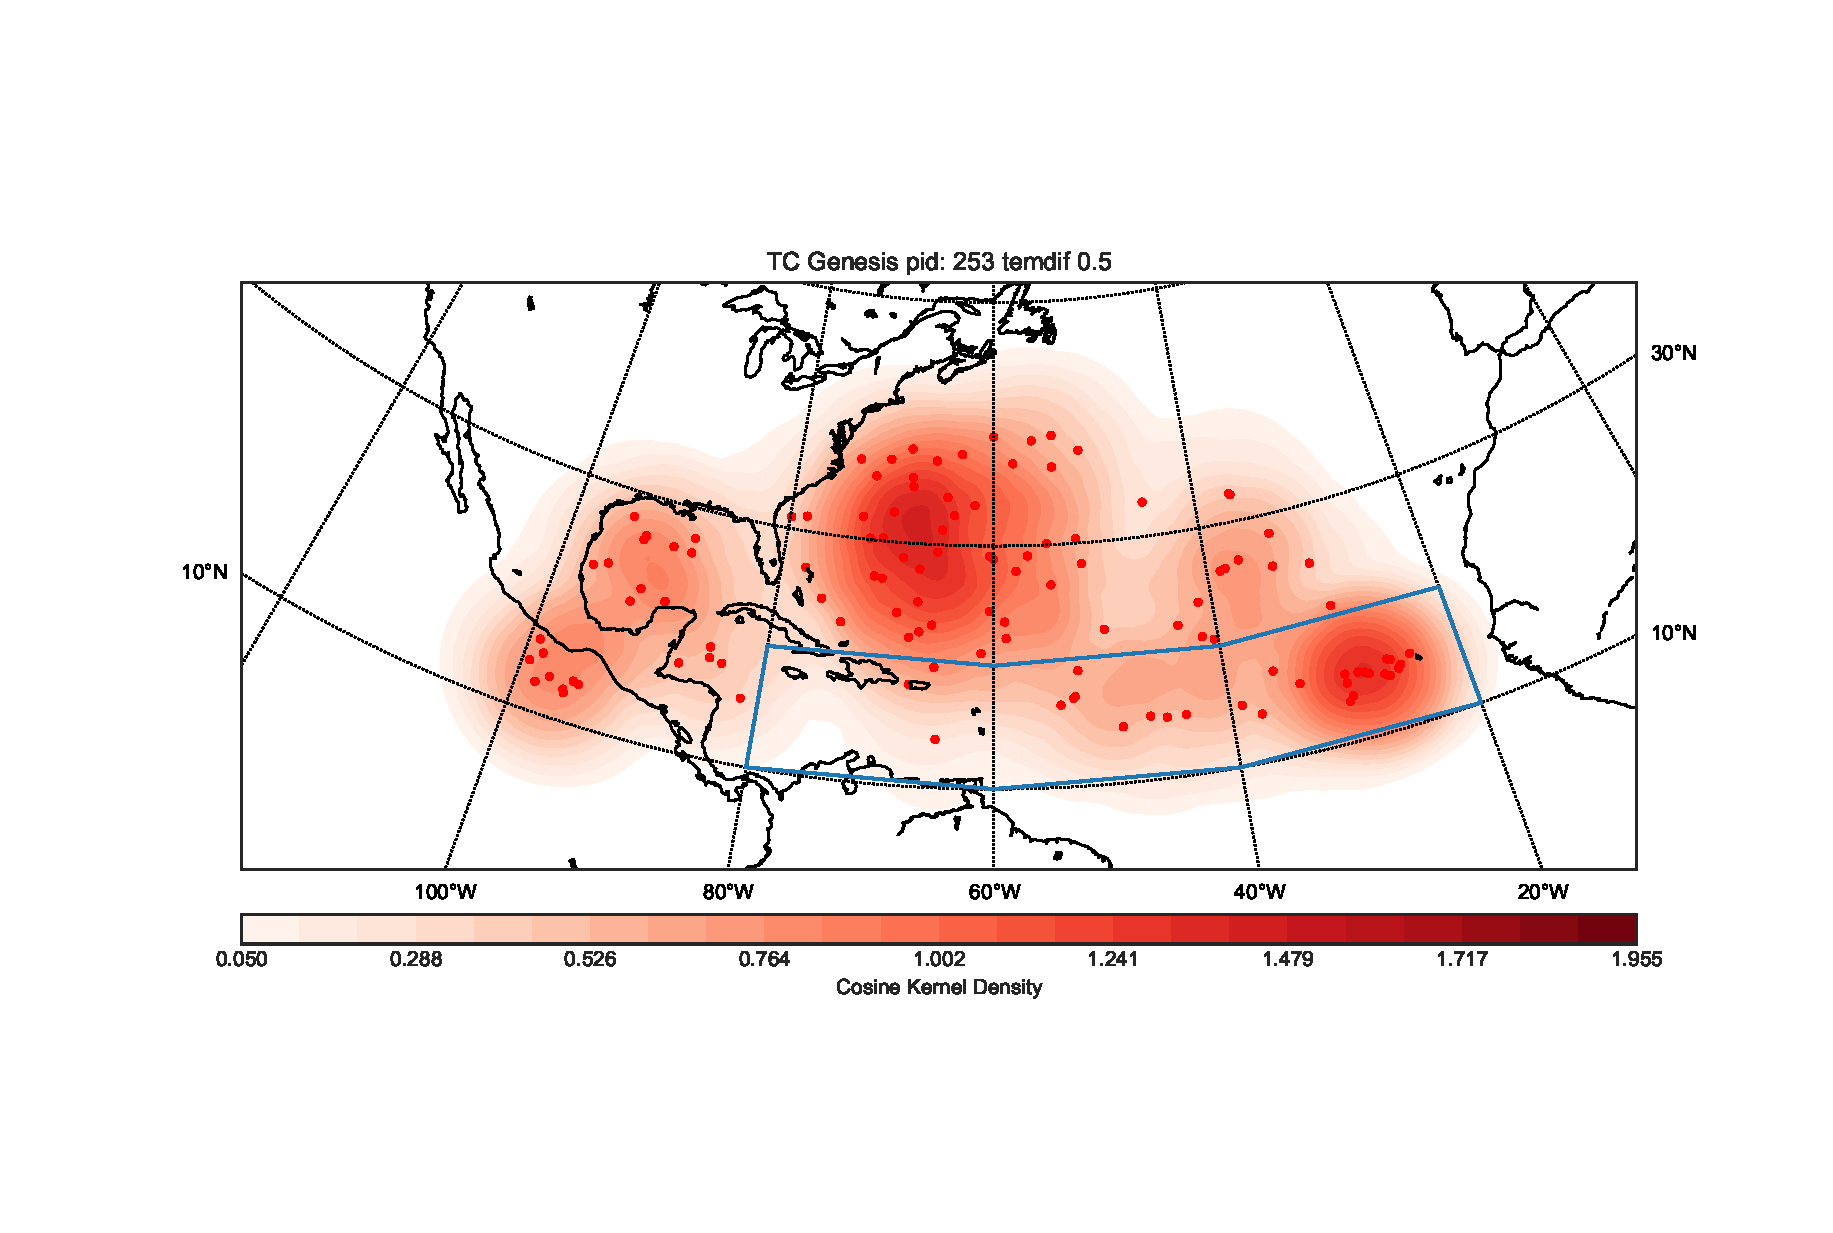
\includegraphics[width=0.7\textwidth]{img/genesis_plot_temdif05.eps}
	\caption{Genesis spots and density for temdif = 0.5.}
\end{figure}
\begin{figure}[ht]
	\centering
	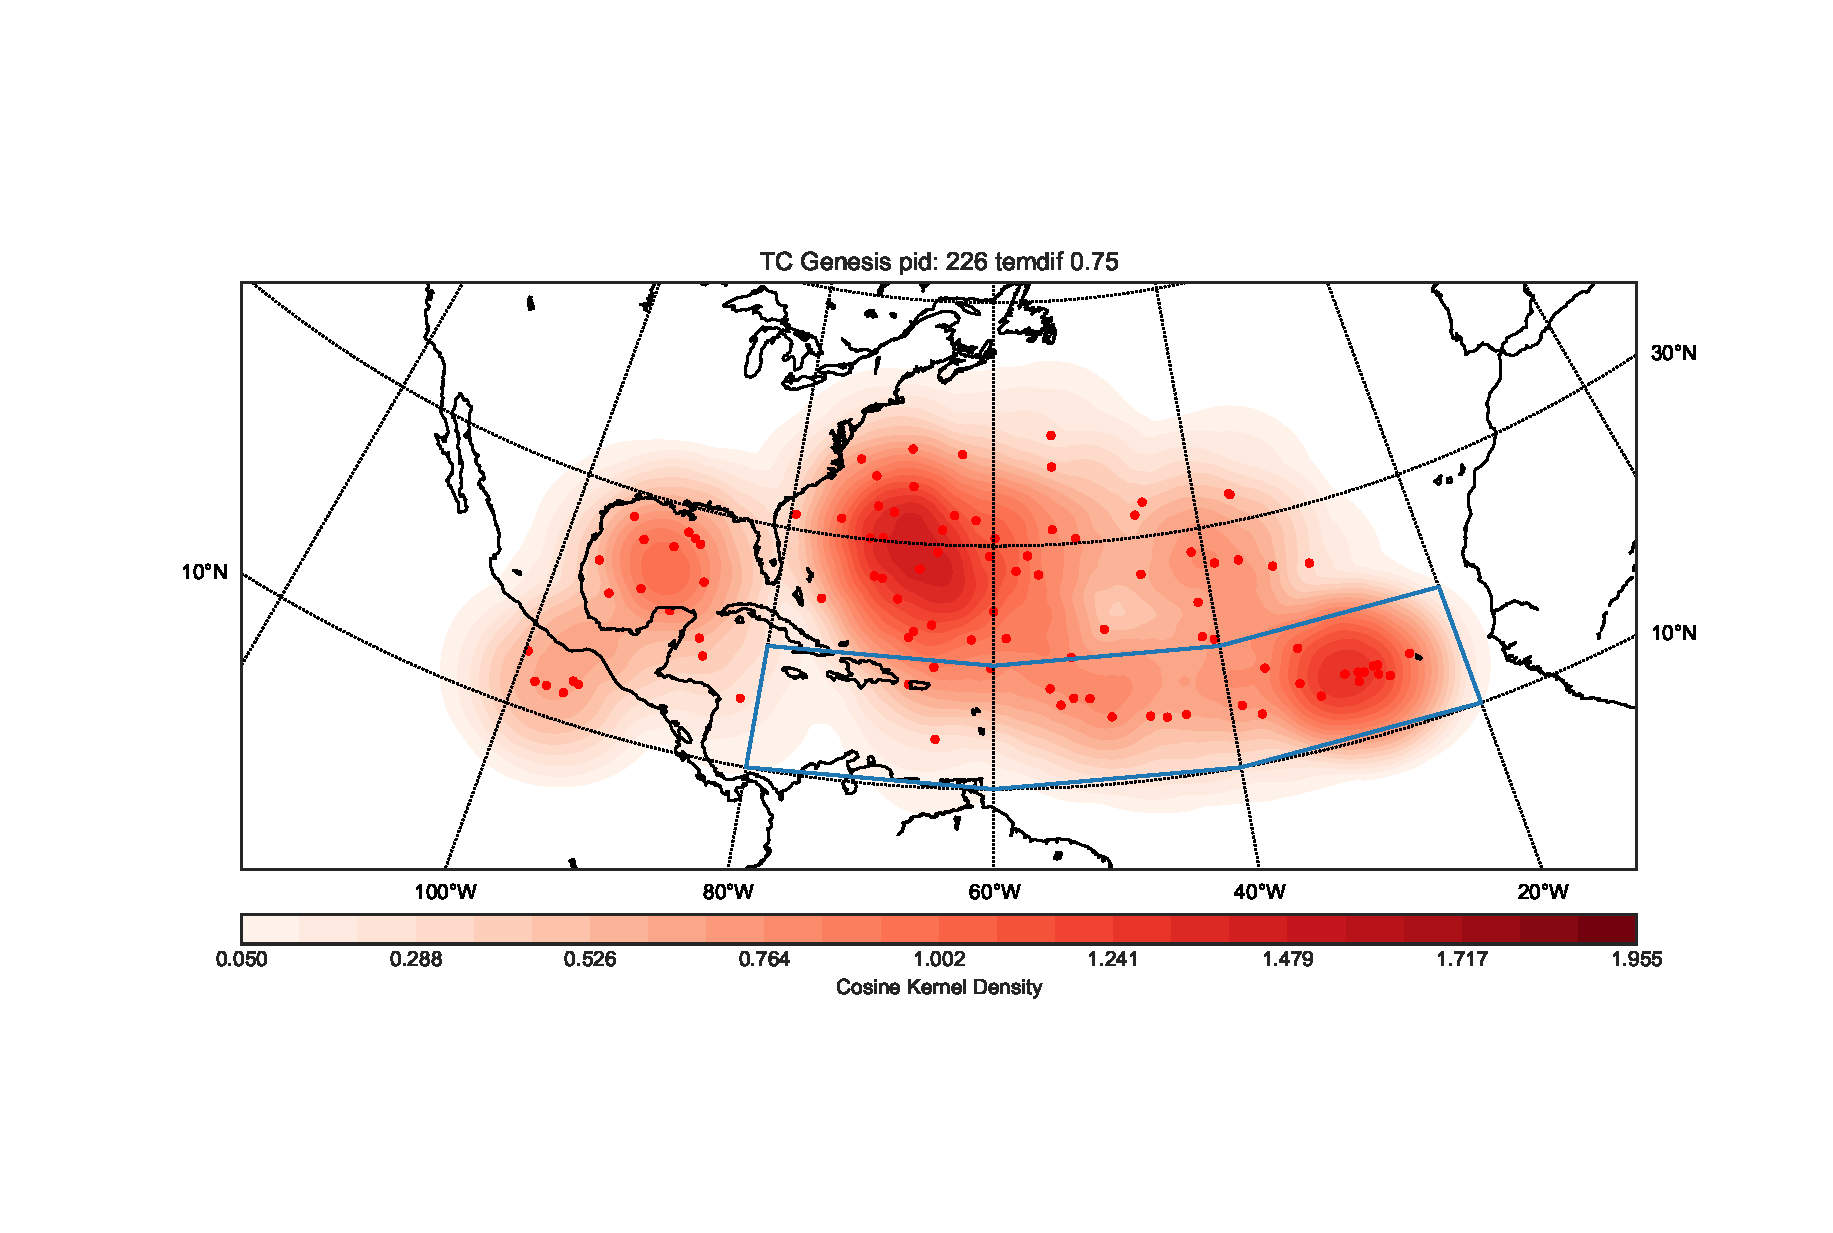
\includegraphics[width=0.7\textwidth]{img/genesis_plot_temdif075.eps}
	\caption{Genesis spots and density for temdif = 0.75.}
\end{figure}
\begin{figure}[ht]
	\centering
	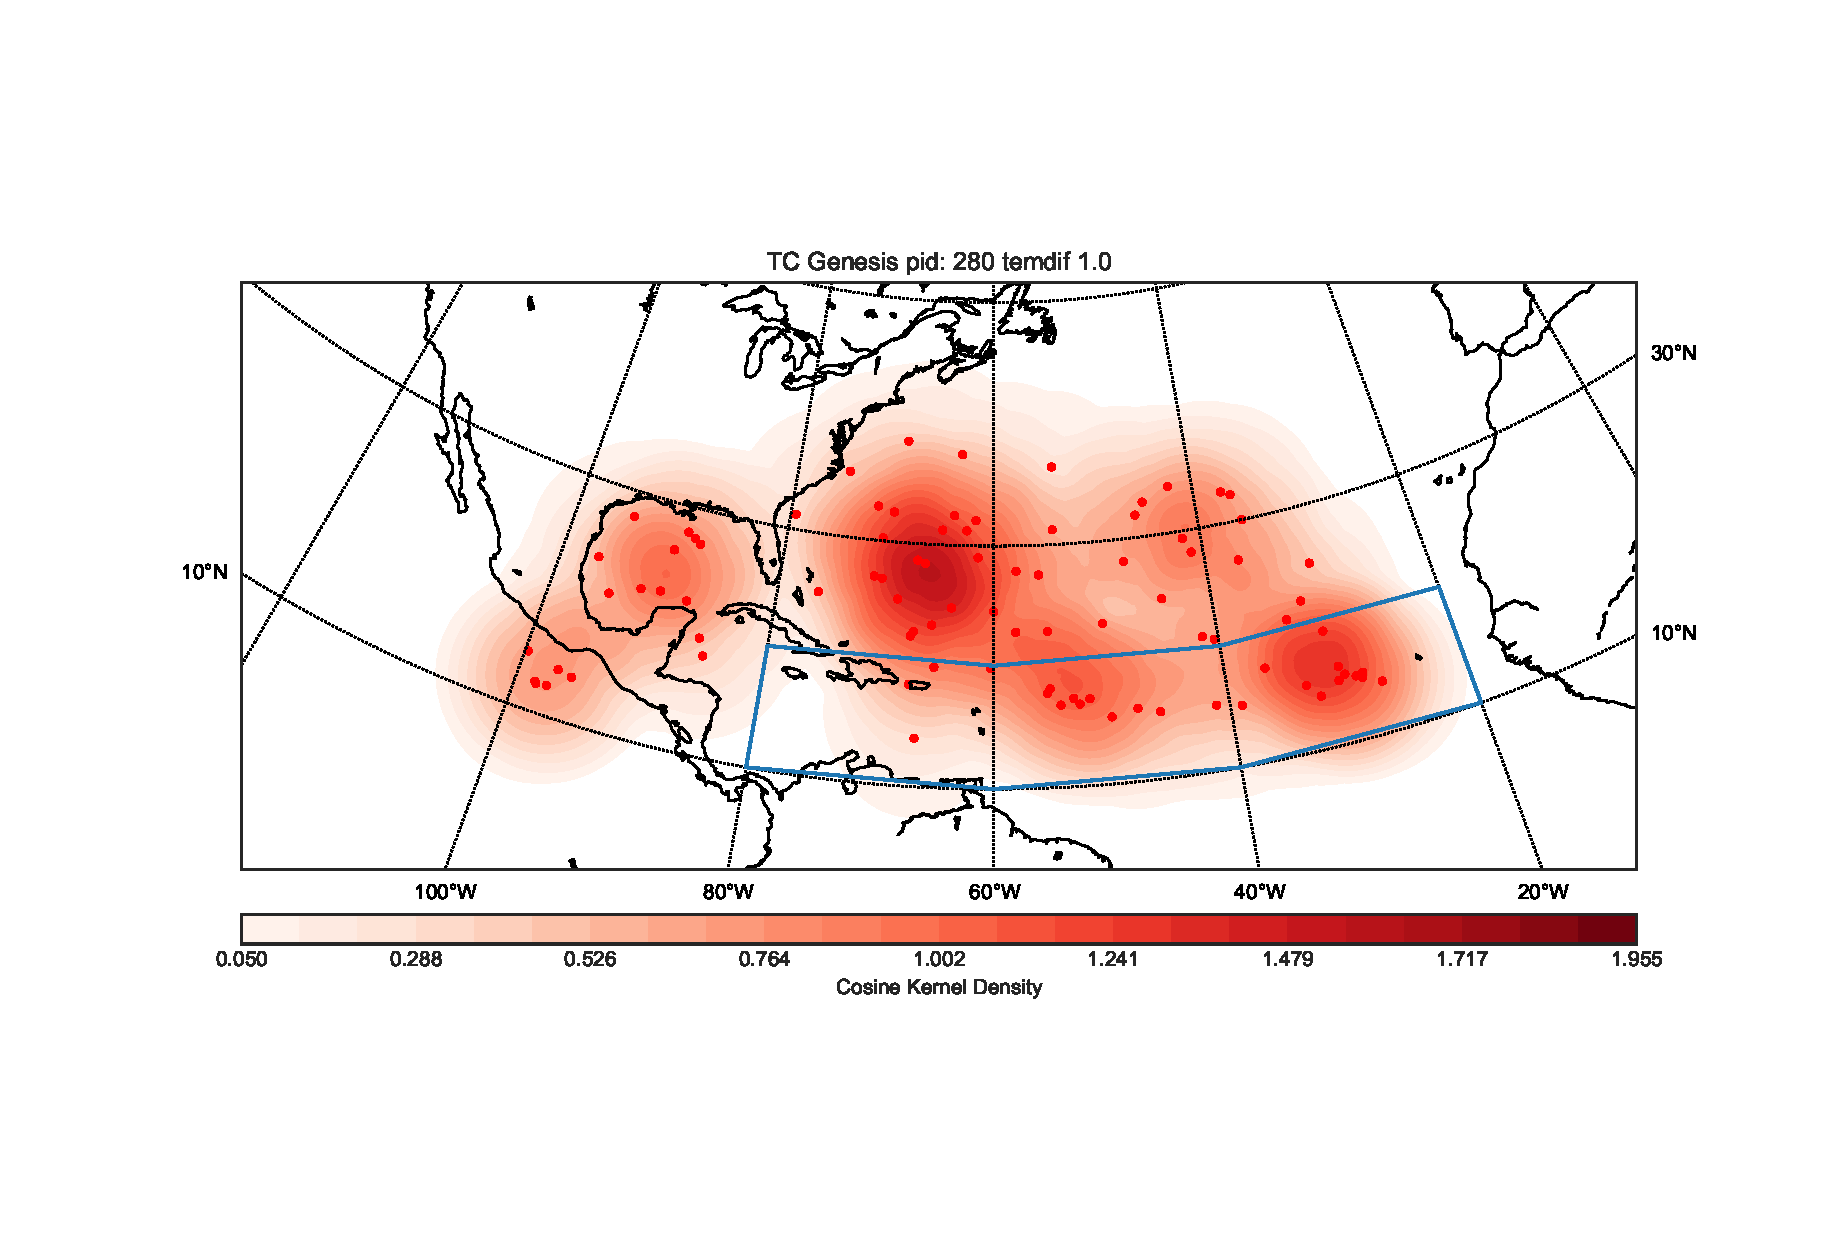
\includegraphics[width=0.7\textwidth]{img/genesis_plot_temdif1.eps}
	\caption{Genesis spots and density for temdif = 1.0.}
\end{figure}
\begin{figure}[ht]
	\centering
	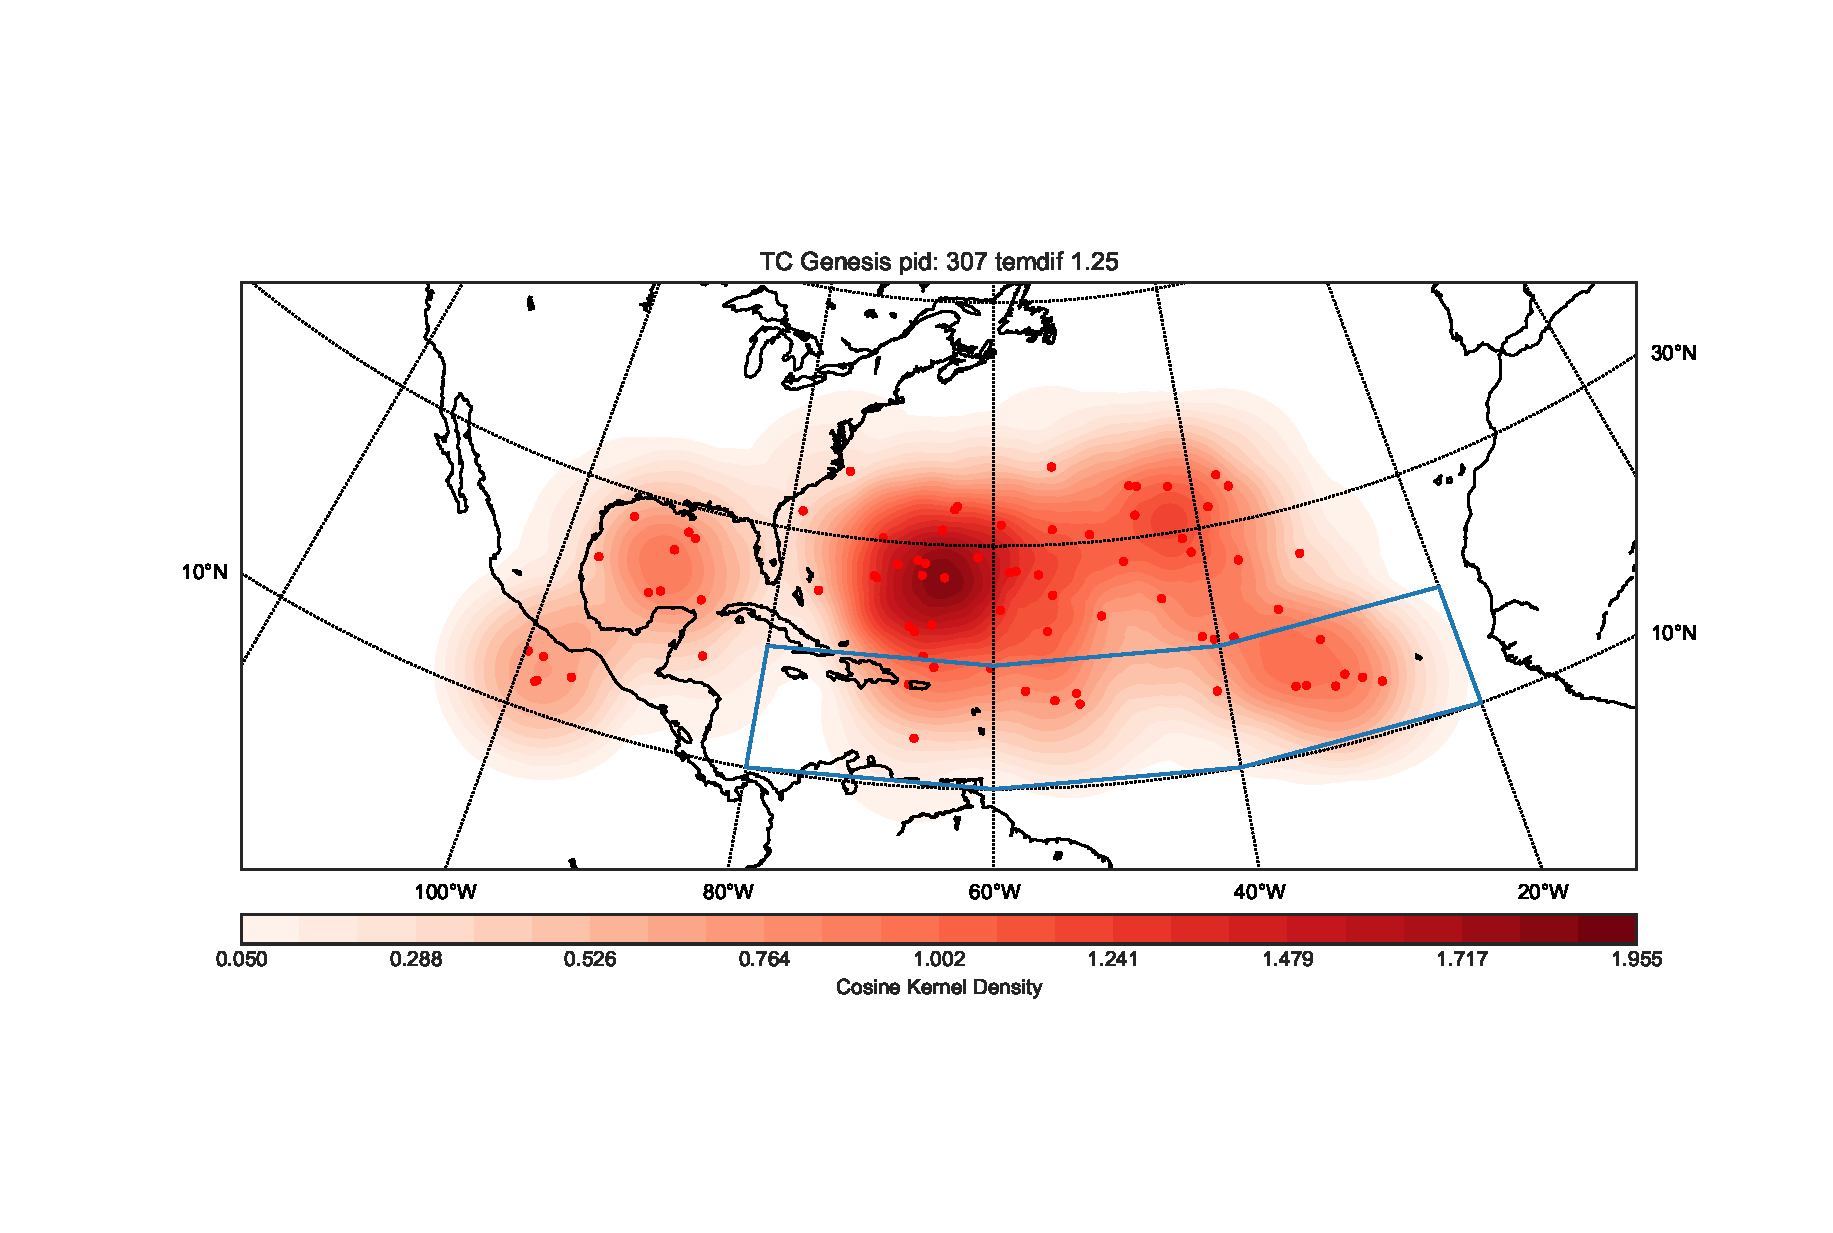
\includegraphics[width=0.7\textwidth]{img/genesis_plot_temdif125.eps}
	\caption{Genesis spots and density for temdif = 1.25.}
\end{figure}
\begin{figure}[ht]
	\centering
	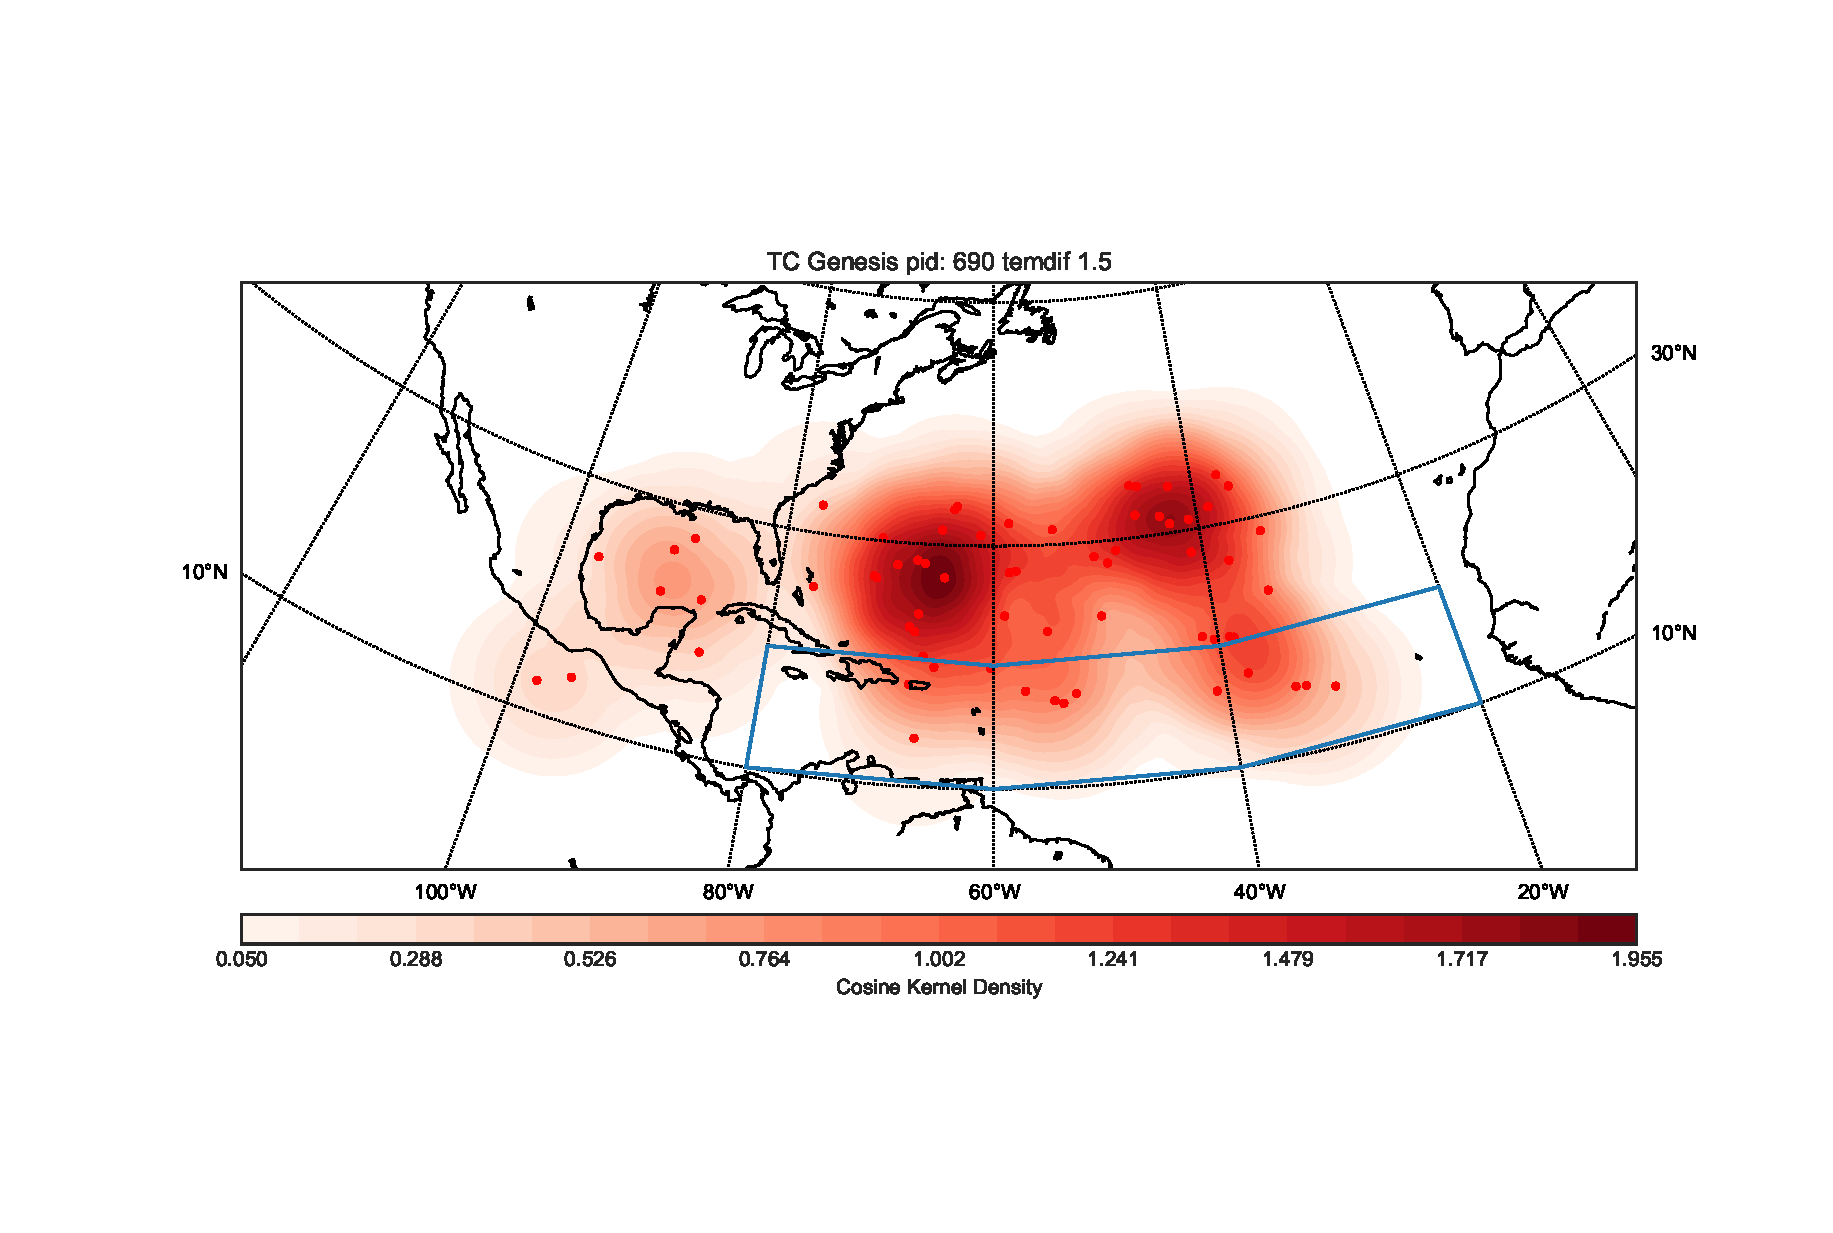
\includegraphics[width=0.7\textwidth]{img/genesis_plot_temdif15.eps}
	\caption{Genesis spots and density for temdif = 1.5.}
\end{figure}

\chapter{Lifetime dependence on the warm core criterion}\label{sec:lifetime-appendix}

\begin{figure}[ht]
	\centering
	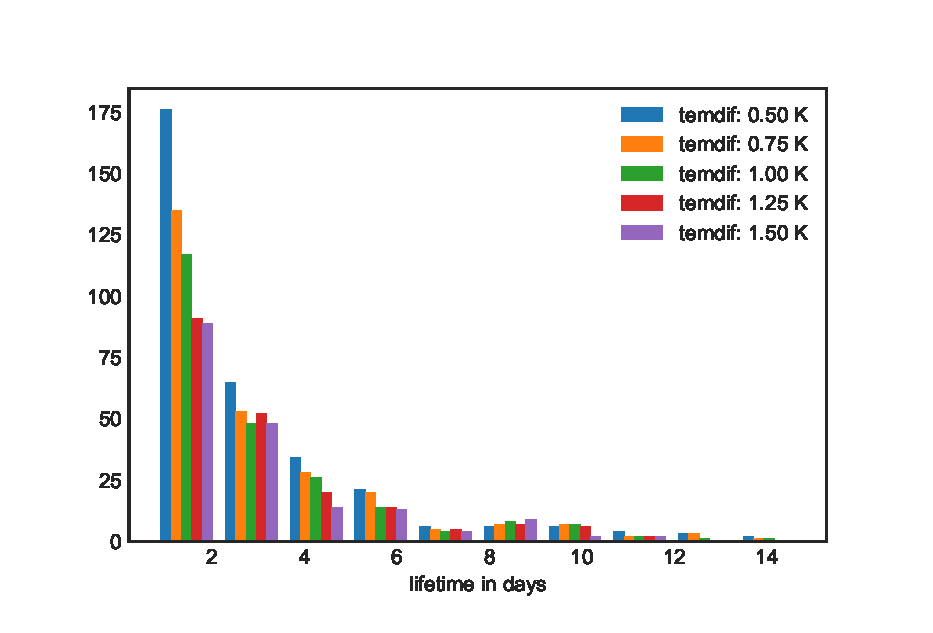
\includegraphics[width=0.7\textwidth]{img/lifetime_for_different_temdif.eps}
	\caption{Histogram showing the number of TCs with a certain lifetime in days.}
\end{figure}

 
 
%---------------------------------------------------------------------------
% Symbols

\chapter*{Nomenclature}\label{chap:symbole}
 \addcontentsline{toc}{chapter}{Nomenclature}
 
\section*{Acronyms and Abbreviations}
\begin{tabbing}
 \hspace*{1.6cm}  \= \kill
 ETH \> Eidgen\"{o}ssische Technische Hochschule \\[0.5ex]
 TC \> Tropical Cyclone \\[0.5ex]
 DWD \> German Weather Service\\[0.5ex]
 MPIM \> Max Planck Institute for Meteorology\\[0.5ex]
ICON \> Icosahedral Nonhydrostatic Model developed by the DWD and the
MPIM\\[0.5ex]
SST \> sea surface temperature\\[0.5ex]
SLP \> sea level pressure\\[0.5ex]
MDR \> main development region  \\[0.5ex]
\end{tabbing}

%---------------------------------------------------------------------------



% Bibliography__________________________________________________________________
% Literature (Additional references can be added to the .bib-file manually, or by using, for example, the free application JabRef). Compile in the following order: latex -bibtex -latex -latex

\bibliographystyle{plain}
\bibliography{bibliography}

\end{document}
